% !TeX root = ../main.tex
% Add the above to each chapter to make compiling the PDF easier in some editors.

\chapter{Implementation}\label{chapter:implementation}
Chapter Introduction


\section{Concept: Features and Interaction Capabilities of the App}
In this section, we explore the expected features and capabilities crucial for our objectives and the necessary interaction capabilities from an end user's perspective.\\
We start with the visualization capabilities of the benchmark data, where the goal is to easily identify performance bottlenecks. This involves pinpointing interesting queries with distinct performances for subsequent in-depth analysis.\\
For deeper analysing and achieving a profound understanding of diverse performance results within queries, the application should support a focus on individual queries. Users should be able to view the performance of a single query from various perspectives, providing a comprehensive image. Comparative analysis across queries from different database systems or even the same database but with different configurations is also essential.\\ 
Then, we examine the requirements for a suitable dashboard that contains the main part of the performance visualizations. Multiple views are necessary to construct a complete understanding of the current point of interest. The optimal structure of these views may vary depending on the point of interest. The flexibility of a drag-and-drop solution for structuring views allows users to tailor the overview according to their specific interests.\\
Finally, we examine the capability of the system to facilitate collaboration and knowledge sharing. The application should enable the saving and sharing of potential findings. This involves saving the interface configuration of the analysis for sharing with other users. Recipients should be able to upload the received configuration, gaining access to the same data and visualization structure for collaborative exploration.


\subsection{Visualising Benchmark Data}
Visualising Benchmark Data includes multiple aspects. It involves the import of the actual data, where a proper way of importing the data should be provided. We also cover the utilized plots and charts for the data visualization. In addition to visualization, we offer a comprehensive table view of the data.


\subsubsection{Charts and Plots}

We aim to offer a dashboard containing multiple data views. To prevent UI clutter, a universal legend of database system instances is suitable, eliminating the necessity to display a legend in every chart. In the legend depicted in Figure~\ref{fig:legend} all database systems included in the benchmark data are presented as colored toggles, allowing users to activate or deactivate their appearance in the visualization. We dive deeper into the interactive legend in \ref{sec:query-analytics}.

\begin{figure}[h]
    \centering
    
\includegraphics[width=1\linewidth]{figures/legend.png}
    \caption{Gobal legend of all database systems contained in the imported performance data.}
    \label{fig:legend}
  \end{figure}



When initiating the analytical process with the Benchy Viewer after importing the benchmark data, it may be beneficial to start with a general and straightforward overview of the benchmark data for quickly gaining an understanding of the general performance standings of the database systems.\\
Within the Benchy Viewer, this overview is effectively conveyed through the relative performance visualization, as depicted in Figure~\ref{fig:relative-performance}. This chart displays, on the Y-Axis, the relative performance of each system in percentage compared to the best-performing system in the benchmark data. The X-Axis lists and represents every database system contained in the benchmark data.

\begin{figure}[h]
  \centering
  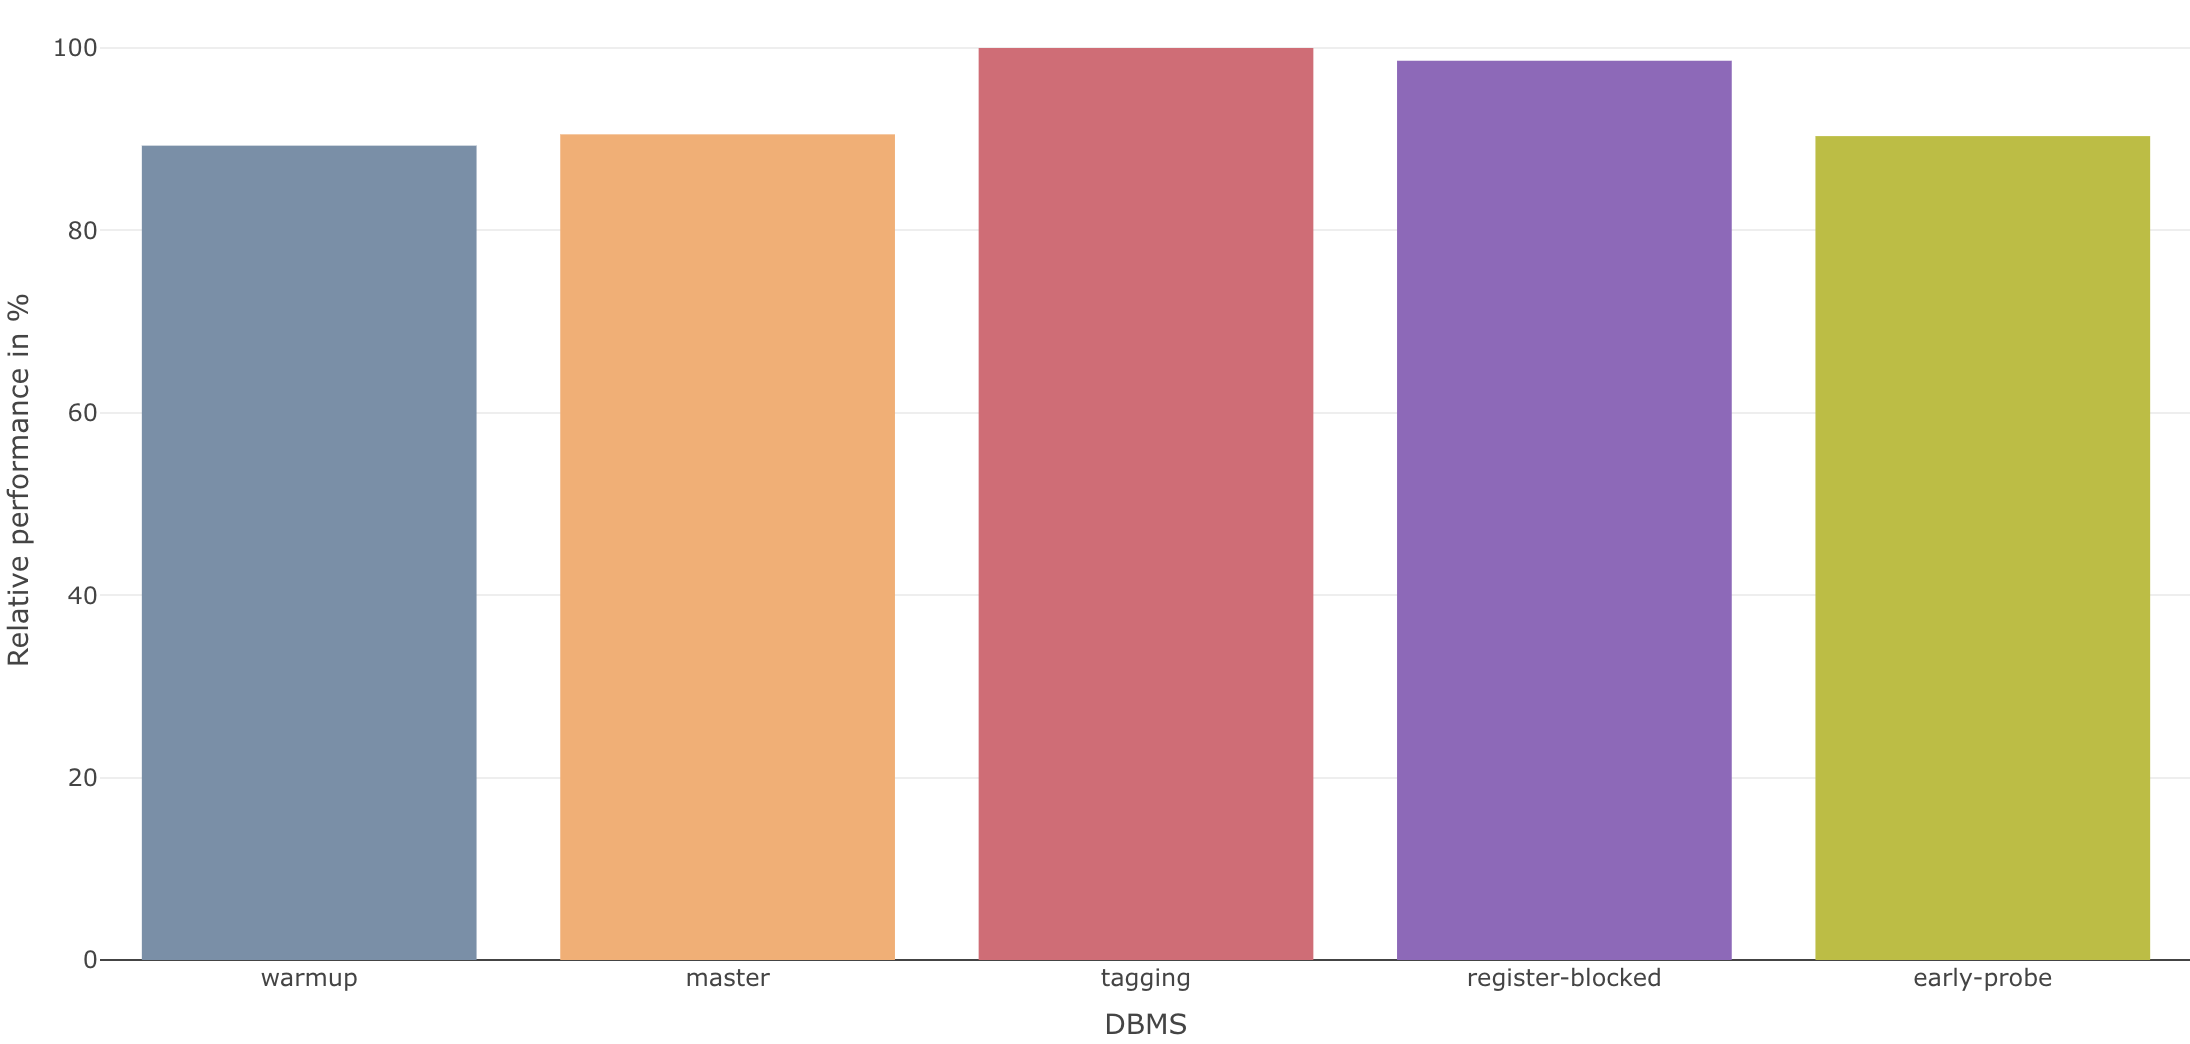
\includegraphics[width=1\linewidth]{figures/bsp-relative-performance.png}
  \caption{Bar chart visualises the relative performance of all systems compared to the best performing system.}
  \label{fig:relative-performance}
\end{figure}

After obtaining this initial overview, users can quickly identify the system marked with the red color as the benchmark, as it processes all queries faster than all other systems. In this visualization, this system is set as the benchmark with 100\% performance, providing a clear reference point for relative comparisons.\\
This chart serves as a valuable starting point for further in-depth analyses and allows users to grasp the overall performance landscape before delving into specific metrics or queries.

In the next phase of the analysis process, we delve into two crucial aspects: compilation and execution. Compilation is the phase where source code is translated into machine code, preparing it for execution Compilation. It is a crucial step that impacts the overall performance of the system. On the other hand, execution is the phase where the compiled code is run on the system. This step involves the actual processing of the instructions and the generation of results. The time spent in the execution phase is a key factor in determining the system's efficiency in handling tasks.

To understand how much time each database system allocates to these processes, the Benchy Viewer offers a stacked bar chart, illustrated in Figure~\ref{fig:execution-compilation}. Here, one section of the bar signifies the time spent in the compilation step, while the other represents the time spent in the execution step.

\begin{figure}[h]
  \centering
  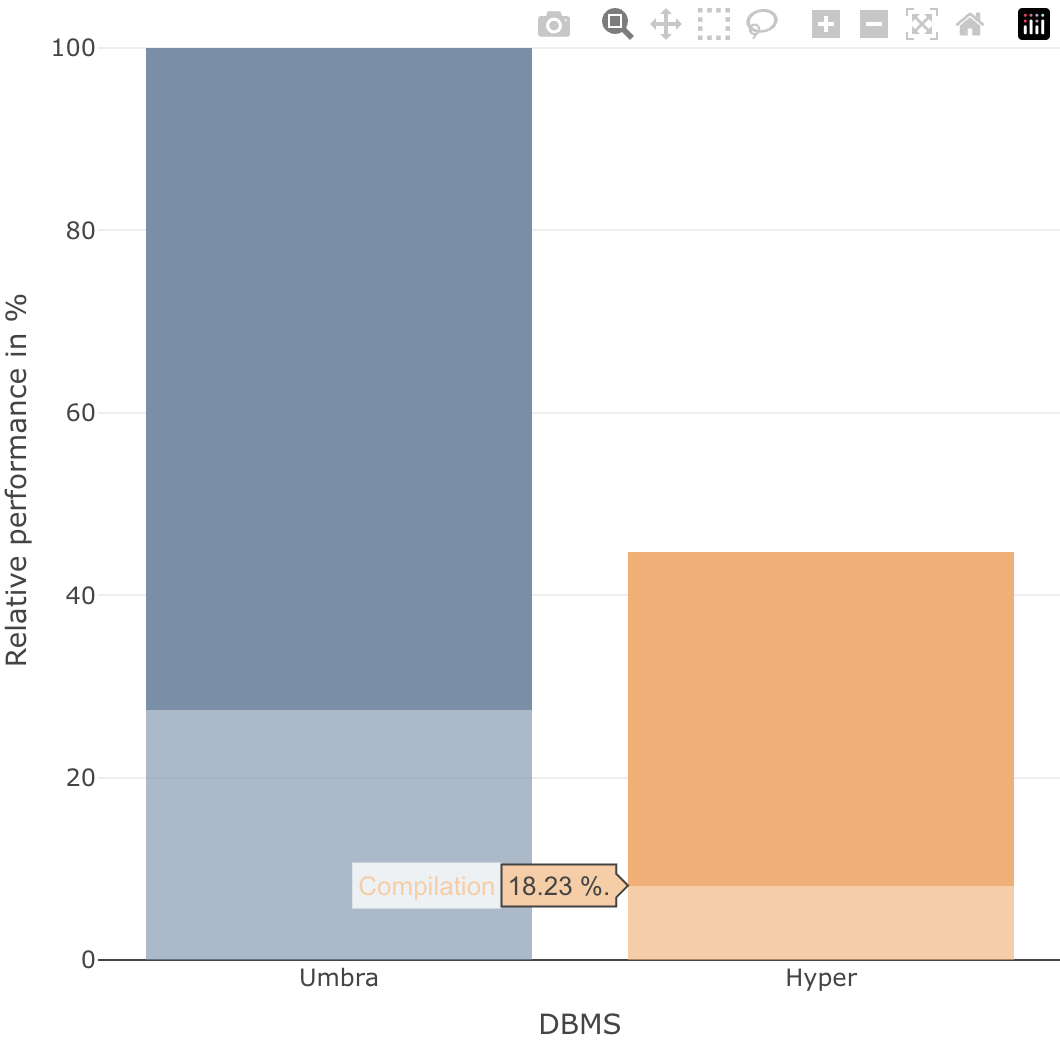
\includegraphics[width=0.5\linewidth]{figures/bsp-compilation-execution.png}
  \caption{Stacked bar chart illustrating the distribution of time between compilation and execution steps. The compilation step is depicted in a transparent accent color, while the execution step is represented in the full color intensity.}
  \label{fig:execution-compilation}
\end{figure}

Using solely the ratio of the two different steps, without taking into account the overall performance, would present an incomplete picture of the balance between the two process steps compared to the better-performing systems. Therefore, this chart complements the relative performance visualization discussed earlier. By incorporating information about the overall performance, it aims to offer a comprehensive understanding while illustrating the equilibrium between compilation and execution for each system.

In this example, a comparison is made between two database systems, with the Y-Axis indicating the relative performance and the X-Axis listing different database systems. Umbra stands out as the best-performing system, with its bar reaching the 100\% level. In contrast, Hyper attains 45\% of Umbra's performance. When hovering over one of the process steps, the chart displays the percentage of the total time spent by the system in that specific step. For instance, Hyper allocated 18.23\% of the entire process to the compilation step, while Umbra spent 27\% on this phase.

Hence, the stacked bar chart in the Benchy Viewer offers a consolidated view of how each database system allocates time between compilation and execution steps. Its integration of the relative performance metric ensures a balanced understanding of system efficiency, preventing oversights from focusing solely on step ratios. With clear visual distinctions and the ability to compare multiple systems, this chart enhances analytical insights into performance disparities and offering an aerial view of compilation and execution.

The preceding visualization solution \textcolor{red}{Referenz auf PDF} shows essential benchmark visualizations, offering both a comprehensive overview of all queries and a detailed examination of each individual query.

It commences with a comparative analysis of each query using a bar chart. Similar to Figure~\ref{fig:bar-chart}, this chart displays queries from various database systems on the X-Axis, with the total time presented on the Y-Axis. 

\begin{figure}[h]
    \centering
    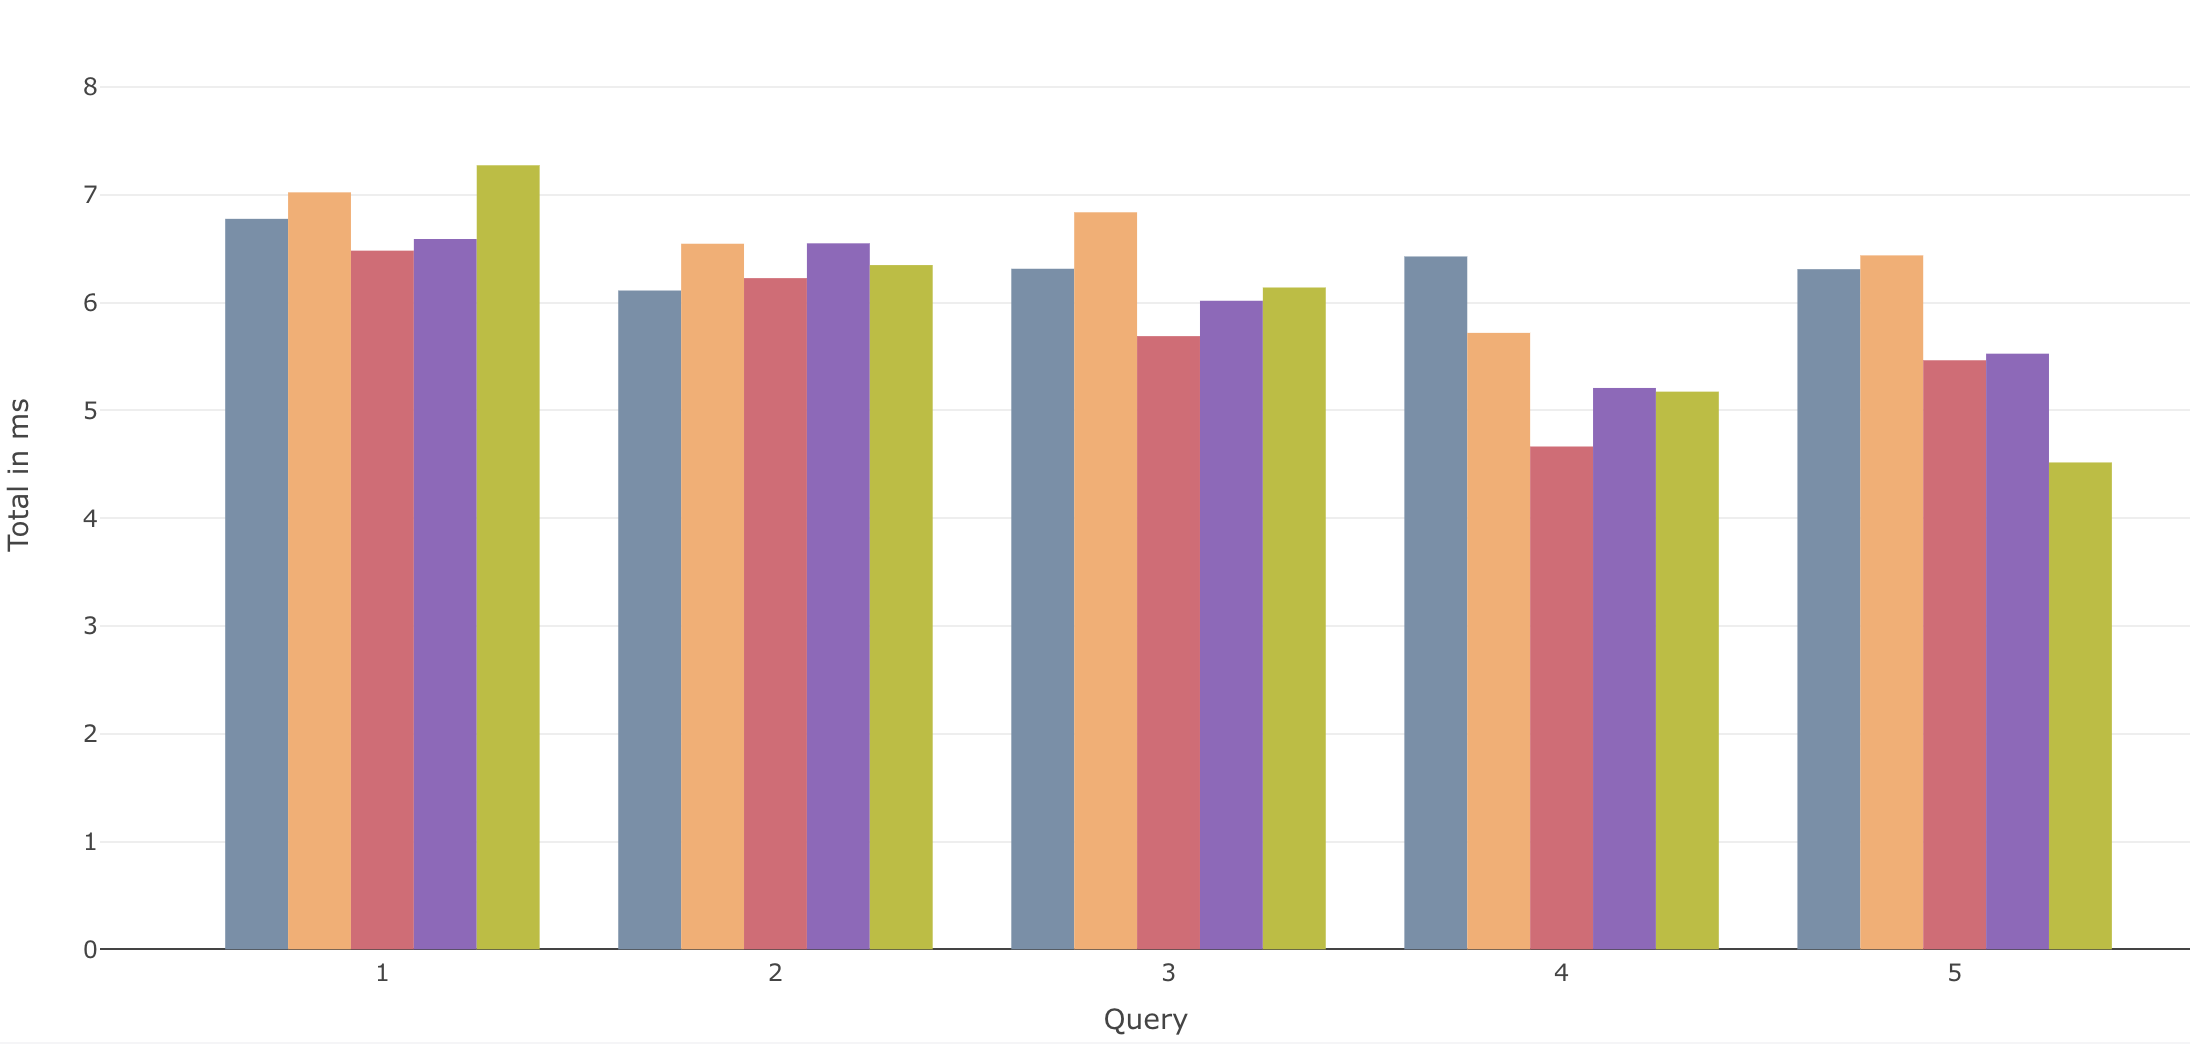
\includegraphics[width=1\linewidth]{figures/bsp-bar.png}
    \caption{Bar chart visualises the totals time in ms of different queries.}
    \label{fig:bar-chart}
  \end{figure}

Bar plots stand out as a versatile visualization method, particularly when tasked with presenting the performance metrics of multiple queries. Their inherent clarity, with the length of each bar directly corresponding to a specific performance metric such as compilation time or execution time, makes them well-suited for diverse scenarios.\\
The straightforward visual comparison they offer is a notable strength. With each query distinctly represented by a separate bar, variations in performance become immediately apparent.\\
This quality proves especially valuable for our objective of identifying outliers, as these exceptional values are easily noticeable.

To facilitate a quick and clear overview of all queries, violin charts are employed. These charts not only provide an initial glimpse of the overall system performance but also offer distribution insights, including the shape and density of the data. They can also be combined with box plots to get a concise summary of the distribution of the results, displaying key statistics such as the median and quartiles.

\begin{figure}[h]
    \centering
    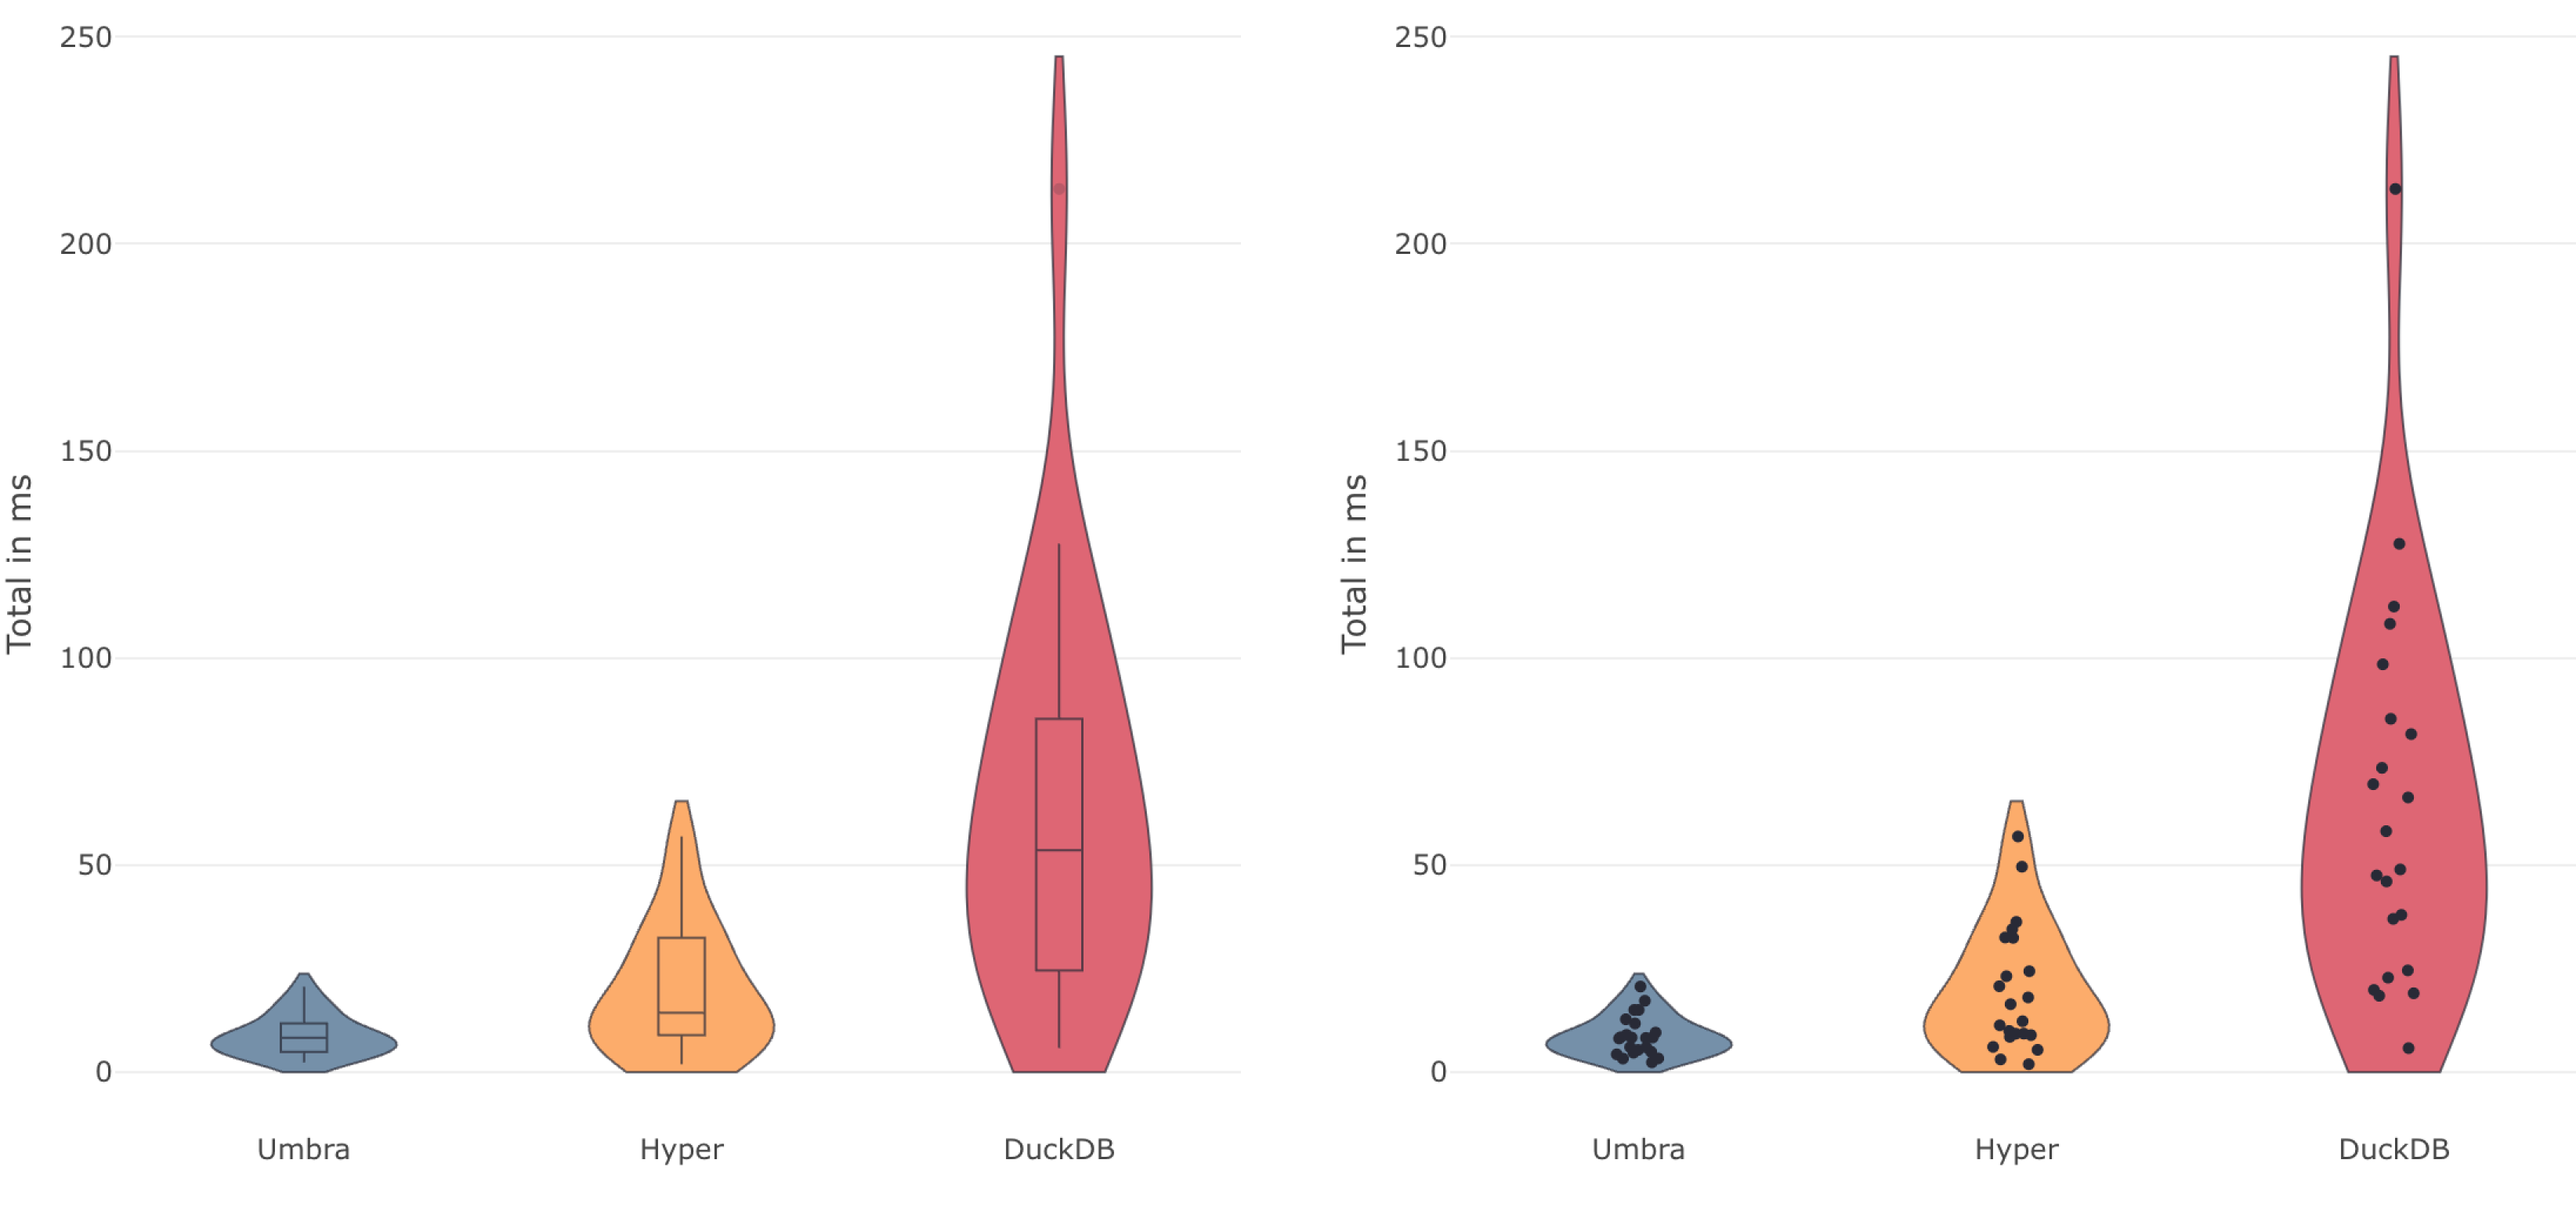
\includegraphics[width=1\linewidth]{figures/bsp-violin-boxplot-points.png}
    \caption{Violin charts visualise the totals time in ms of different queries. The left variant contains a box plot and the right variant contains all data points.}
    \label{fig:violin-chart}
  \end{figure}

Within the Benchy Viewer violin plots that contain data points, as shown in Figure~\ref{fig:violin-chart} on the right side, additionally allow you to hover over a data point. This action highlights the corresponding query in the violins of the other database systems. We will explore this hover feature further in \ref{sec:hover-feature}.


Conducting benchmark performance analysis often necessitates a comparative approach between a chosen system and other competing systems. The Benchy Viewer facilitates this by enabling the selection of a baseline system from one of the database systems included in the benchmark data, as shown in Figure~\ref{fig:select-baseline-system}.

\begin{figure}[h]
  \centering
  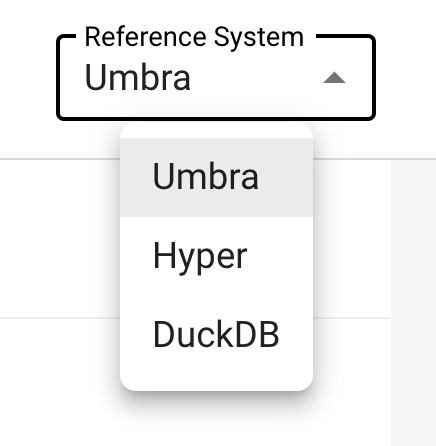
\includegraphics[width=0.3\linewidth]{figures/select-baseline-system.png}
  \caption{A drop-down menu that allows to select a baseline system.}
  \label{fig:select-baseline-system}
\end{figure}


This functionality proves useful for assessing how the performance of the chosen baseline system compares to others, aiding in the identification of strengths, weaknesses, and potential optimization areas. It forms a foundational step in the detailed analysis provided by the Benchy Viewer. Several visualizations in the application utilize the baseline system, including the table view and scatter plot for inspecting the slow-down and speedup metric, and the bar chart showcasing the performance delta for each query from the perspective of the baseline system. All these visualizations depend on a baseline system, making this functionality crucial for a comprehensive performance analysis.

In the context of providing a clear and comparative understanding of how different systems perform relative to a chosen baseline, the metrics maximum slow-down and maximum speedup become crucial. They offer a comprehensive view of the range of performance variations. Maximum slow-down indicates the worst-case scenario of reduced performance, while maximum speedup highlights the most significant improvement achieved.

\textbf{Slowdown} indicates how much slower a specific system is compared to the baseline system. It is calculated as the ratio of the time taken by the system under consideration to the time taken by the baseline system. A slow-down value greater than 1 implies that the system is slower than the baseline. For example, a slow-down of 1.5 means the system is 1.5 times slower than the baseline.\\
Identifying slow-downs is crucial for pinpointing areas of inefficiency or performance bottlenecks in a system. It helps in understanding where improvements are needed.

\textbf{Speedup}, on the other hand, quantifies how much faster a specific system is compared to the baseline system. It is calculated similarly to slow-down but in the reverse manner. A speedup value greater than 1 implies that the system is faster than the baseline. For example, a speedup of 2 means the system is twice as fast as the baseline.\\
Knowing the speedup is essential to highlight improvements. It indicates the effectiveness of optimizations or enhancements made to the system compared to the baseline.

The Benchy Viewer employs tables to showcase the maximum slow-down and maximum speedup, visualised in Figure~\ref{fig:slowdown-speedup-chart}, where the maximum slow-down is displayed on the left side and the maximum speedup on the right side using Umbra as the baseline system. The use of cell colors in the table serves as an effective visual indicator of performance outliers. Intensity in color corresponds to the extent of the outlier, offering a rapid understanding of the range and distribution between these extreme values. This color-coded representation aids users in identifying and assessing the significance of performance variations across different systems.

\begin{figure}[h]
  \centering
  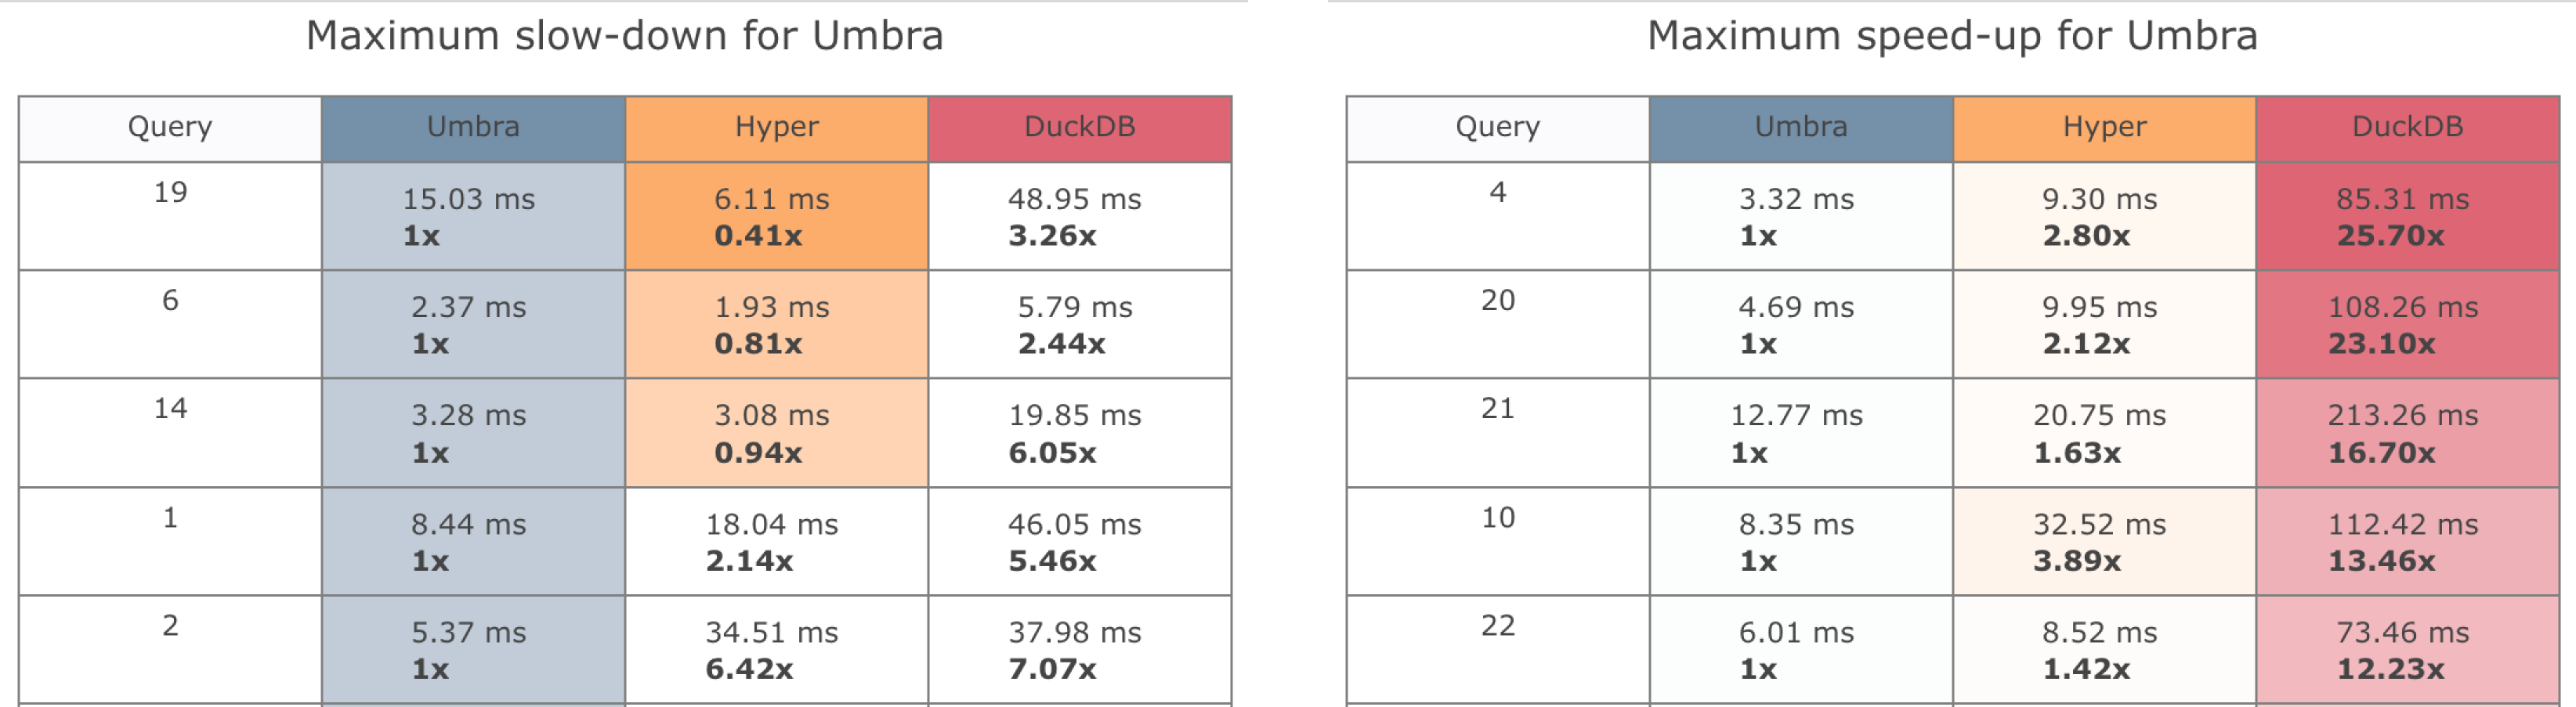
\includegraphics[width=1\linewidth]{figures/bsp-table-speedup-slowdown.png}
  \caption{Tables showcase the maximum slow-down and the maximum speedup using color intensity to indicate performance outliers.}
  \label{fig:slowdown-speedup-chart}
\end{figure}

The tables are organized based on the resulting ratio.\\
In the maximum slow-down tables, the arrangement is ascending, placing the slowest queries of the baseline system compared to the faster alternative system at the top.\\
Conversely, in maximum speedup tables, the sorting is descending, presenting the fastest queries of the baseline system compared to the alternative system at the forefront. This sorting strategy provides a logical structure to quickly identify and compare performance differences in either scenario.

The scatter plot is another effective choice for visualising speedup and slow-down. These plots are particularly beneficial for trend analysis, offering a detailed view of each query individually. Users can identify trends, clusters, or outliers in the data, providing insights that might be less apparent in a table.

In the Benchy Viewer a baseline is displayed, as illustrated in Figure~\ref{fig:scatter} positioned at Y = 1 and colored in blue. This positioning allows users to observe the relative performance of each query compared to the baseline system.

\begin{figure}[h]
  \centering
  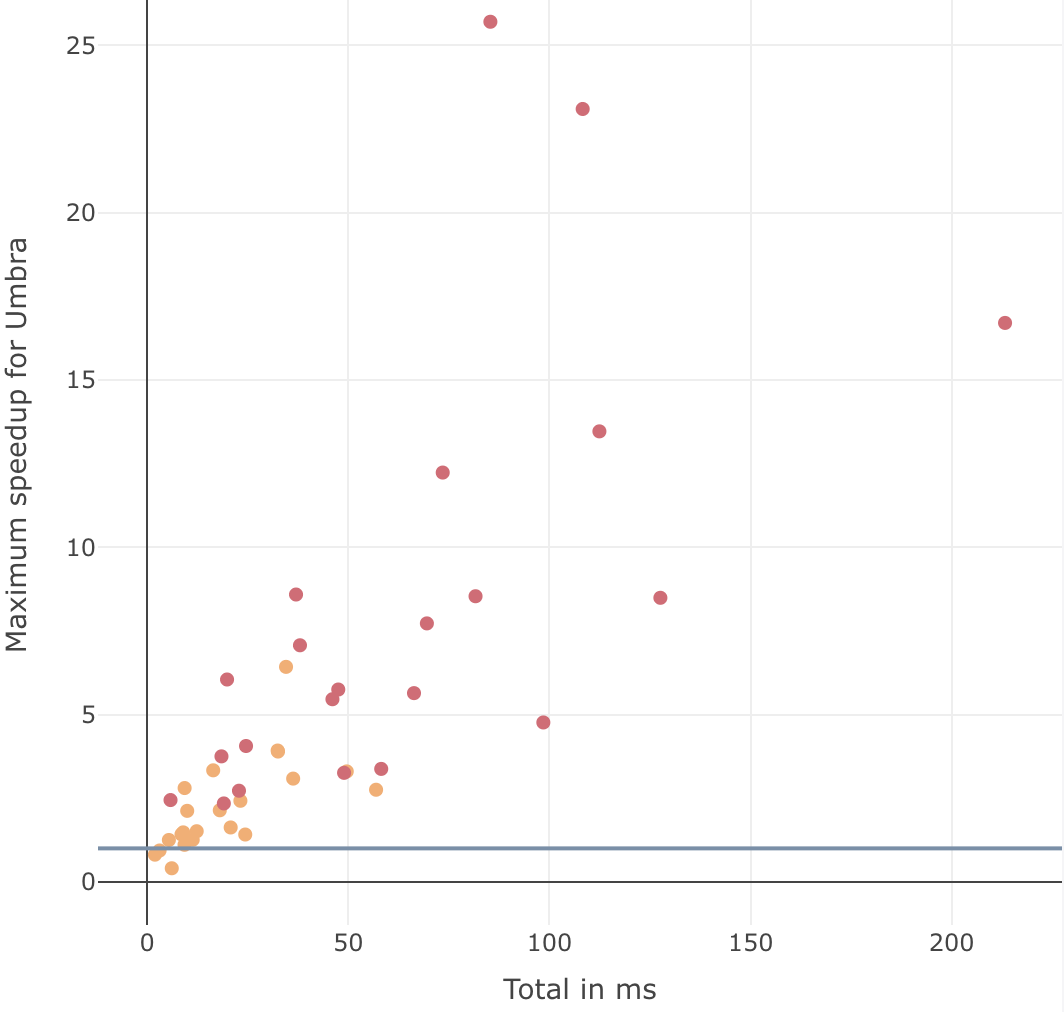
\includegraphics[width=0.7\linewidth]{figures/bsp-scatter.png}
  \caption{Scatter Plot visualises the speedup.}
  \label{fig:scatter}
\end{figure}

In this example, the scatter plot represents the maximum speedup for the selected baseline system on the Y-axis, while the total time in milliseconds is represented on the X-axis. This visualises the relationship between the total time taken by each query and its corresponding speedup compared to the baseline system.\\
Hovering above these query data points reveals the ratio of the corresponding speedup and the query identifier. We will explore the hover feature further in \ref{sec:hover-feature}.\\
Queries from the competing system are marked in orange, and most of them are slower, with three queries below the baseline, indicating that these particular queries are faster.\\
This observation prompts further investigation into the queries below the baseline, offering an opportunity to identify potential performance bottlenecks from the perspective of the baseline system. This nuanced understanding, facilitated by the visual representation of the scatter plot, guides users in pinpointing specific queries that deviate from the expected performance trend, aiding in targeted optimizations and analysis.

In the Benchy Viewer, another visualization occurs, highlighting the performance disparities between a chosen baseline system and its competitors. It takes the form of a bar chart that illustrates the performance gap for each query, providing a perspective of the baseline system compared to the best-performing query of other competing systems.

The performance delta chart in the Benchy Viewer not only displays the performance gap for each query from the perspective of the baseline system but also indicates the best competing system for each query by using corresponding system colors, as depicted in Figure~\ref{fig:performance-gap}. The Y-axis shows the performance gap percentage of the competing queries, while the X-axis represents the identifying query number. Hovering over bars reveals the exact performance delta.

\begin{figure}[h]
  \centering
  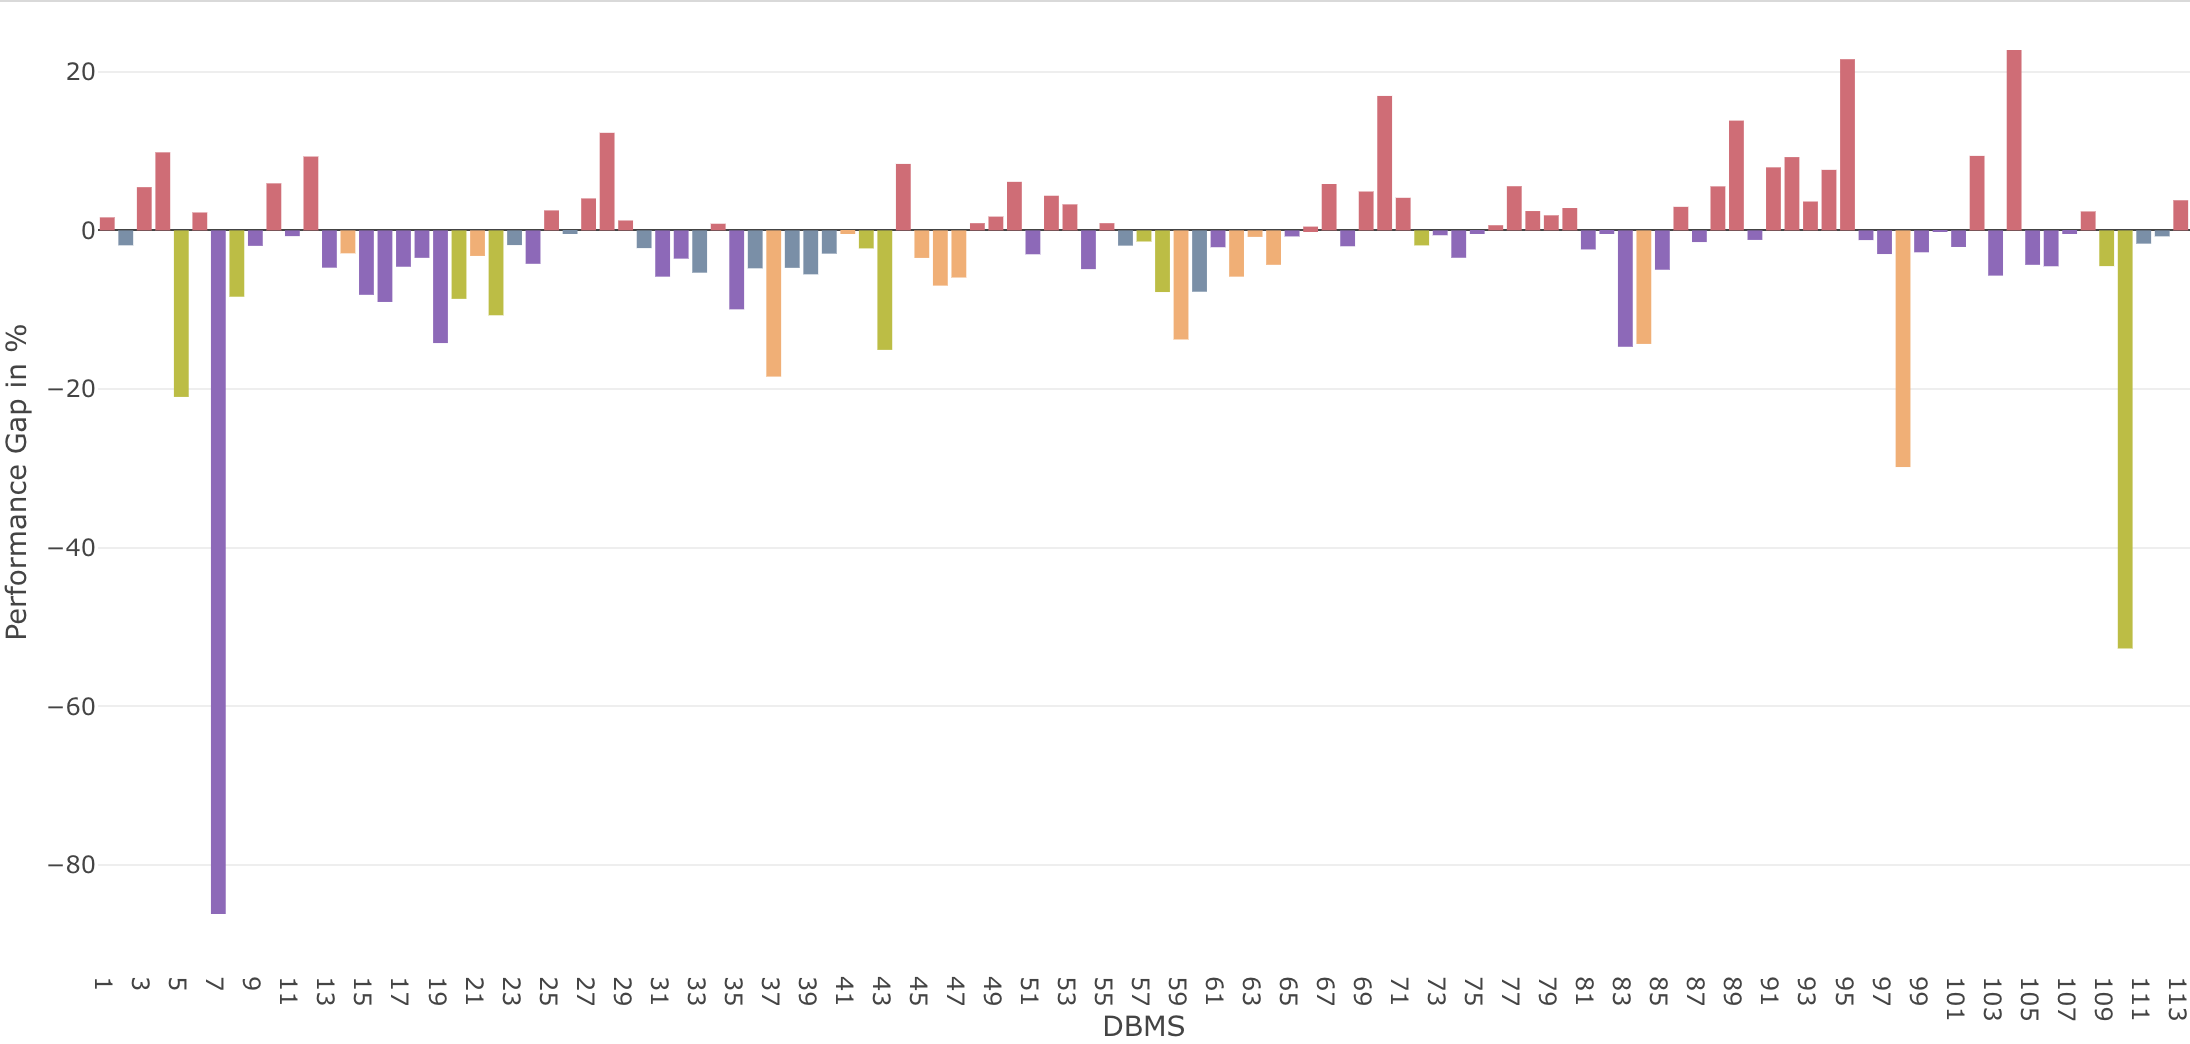
\includegraphics[width=1\linewidth]{figures/bsp-query-gaps.png}
  \caption{Bar chart visualises the performance gap for every query of the baseline system compared to best corresponding query of the competing systems.}
  \label{fig:performance-gap}
\end{figure}

In this example, the red-marked database system is selected as the baseline system. Queries with faster performance by the baseline system are displayed above the baseline, indicating a positive performance delta. In contrast, queries with stronger performance by competing systems are shown below the baseline, indicating a negative performance delta for the baseline system. Additionally, the bar of each query is marked with the color of the corresponding best-performing database system.\\
The performance gap for the majority of cases in this example stays within a range between -20\% and 20\%. However, some outliers are notably significant. For instance, the seventh query has a performance gap of -86\%. A deeper analysis of this query may be sensible to potentially identify performance bottlenecks from the perspective of the baseline system.

This query performance gap visualization is instrumental in quickly discerning how each query of the baseline system stacks up against the top-performing queries of other systems. The chart's simplicity ensures easy comprehension, enabling users to promptly assess the relative performance of different queries.




\subsubsection{Hover Feature}\label{sec:hover-feature}

\begin{figure}[h]
  \centering
  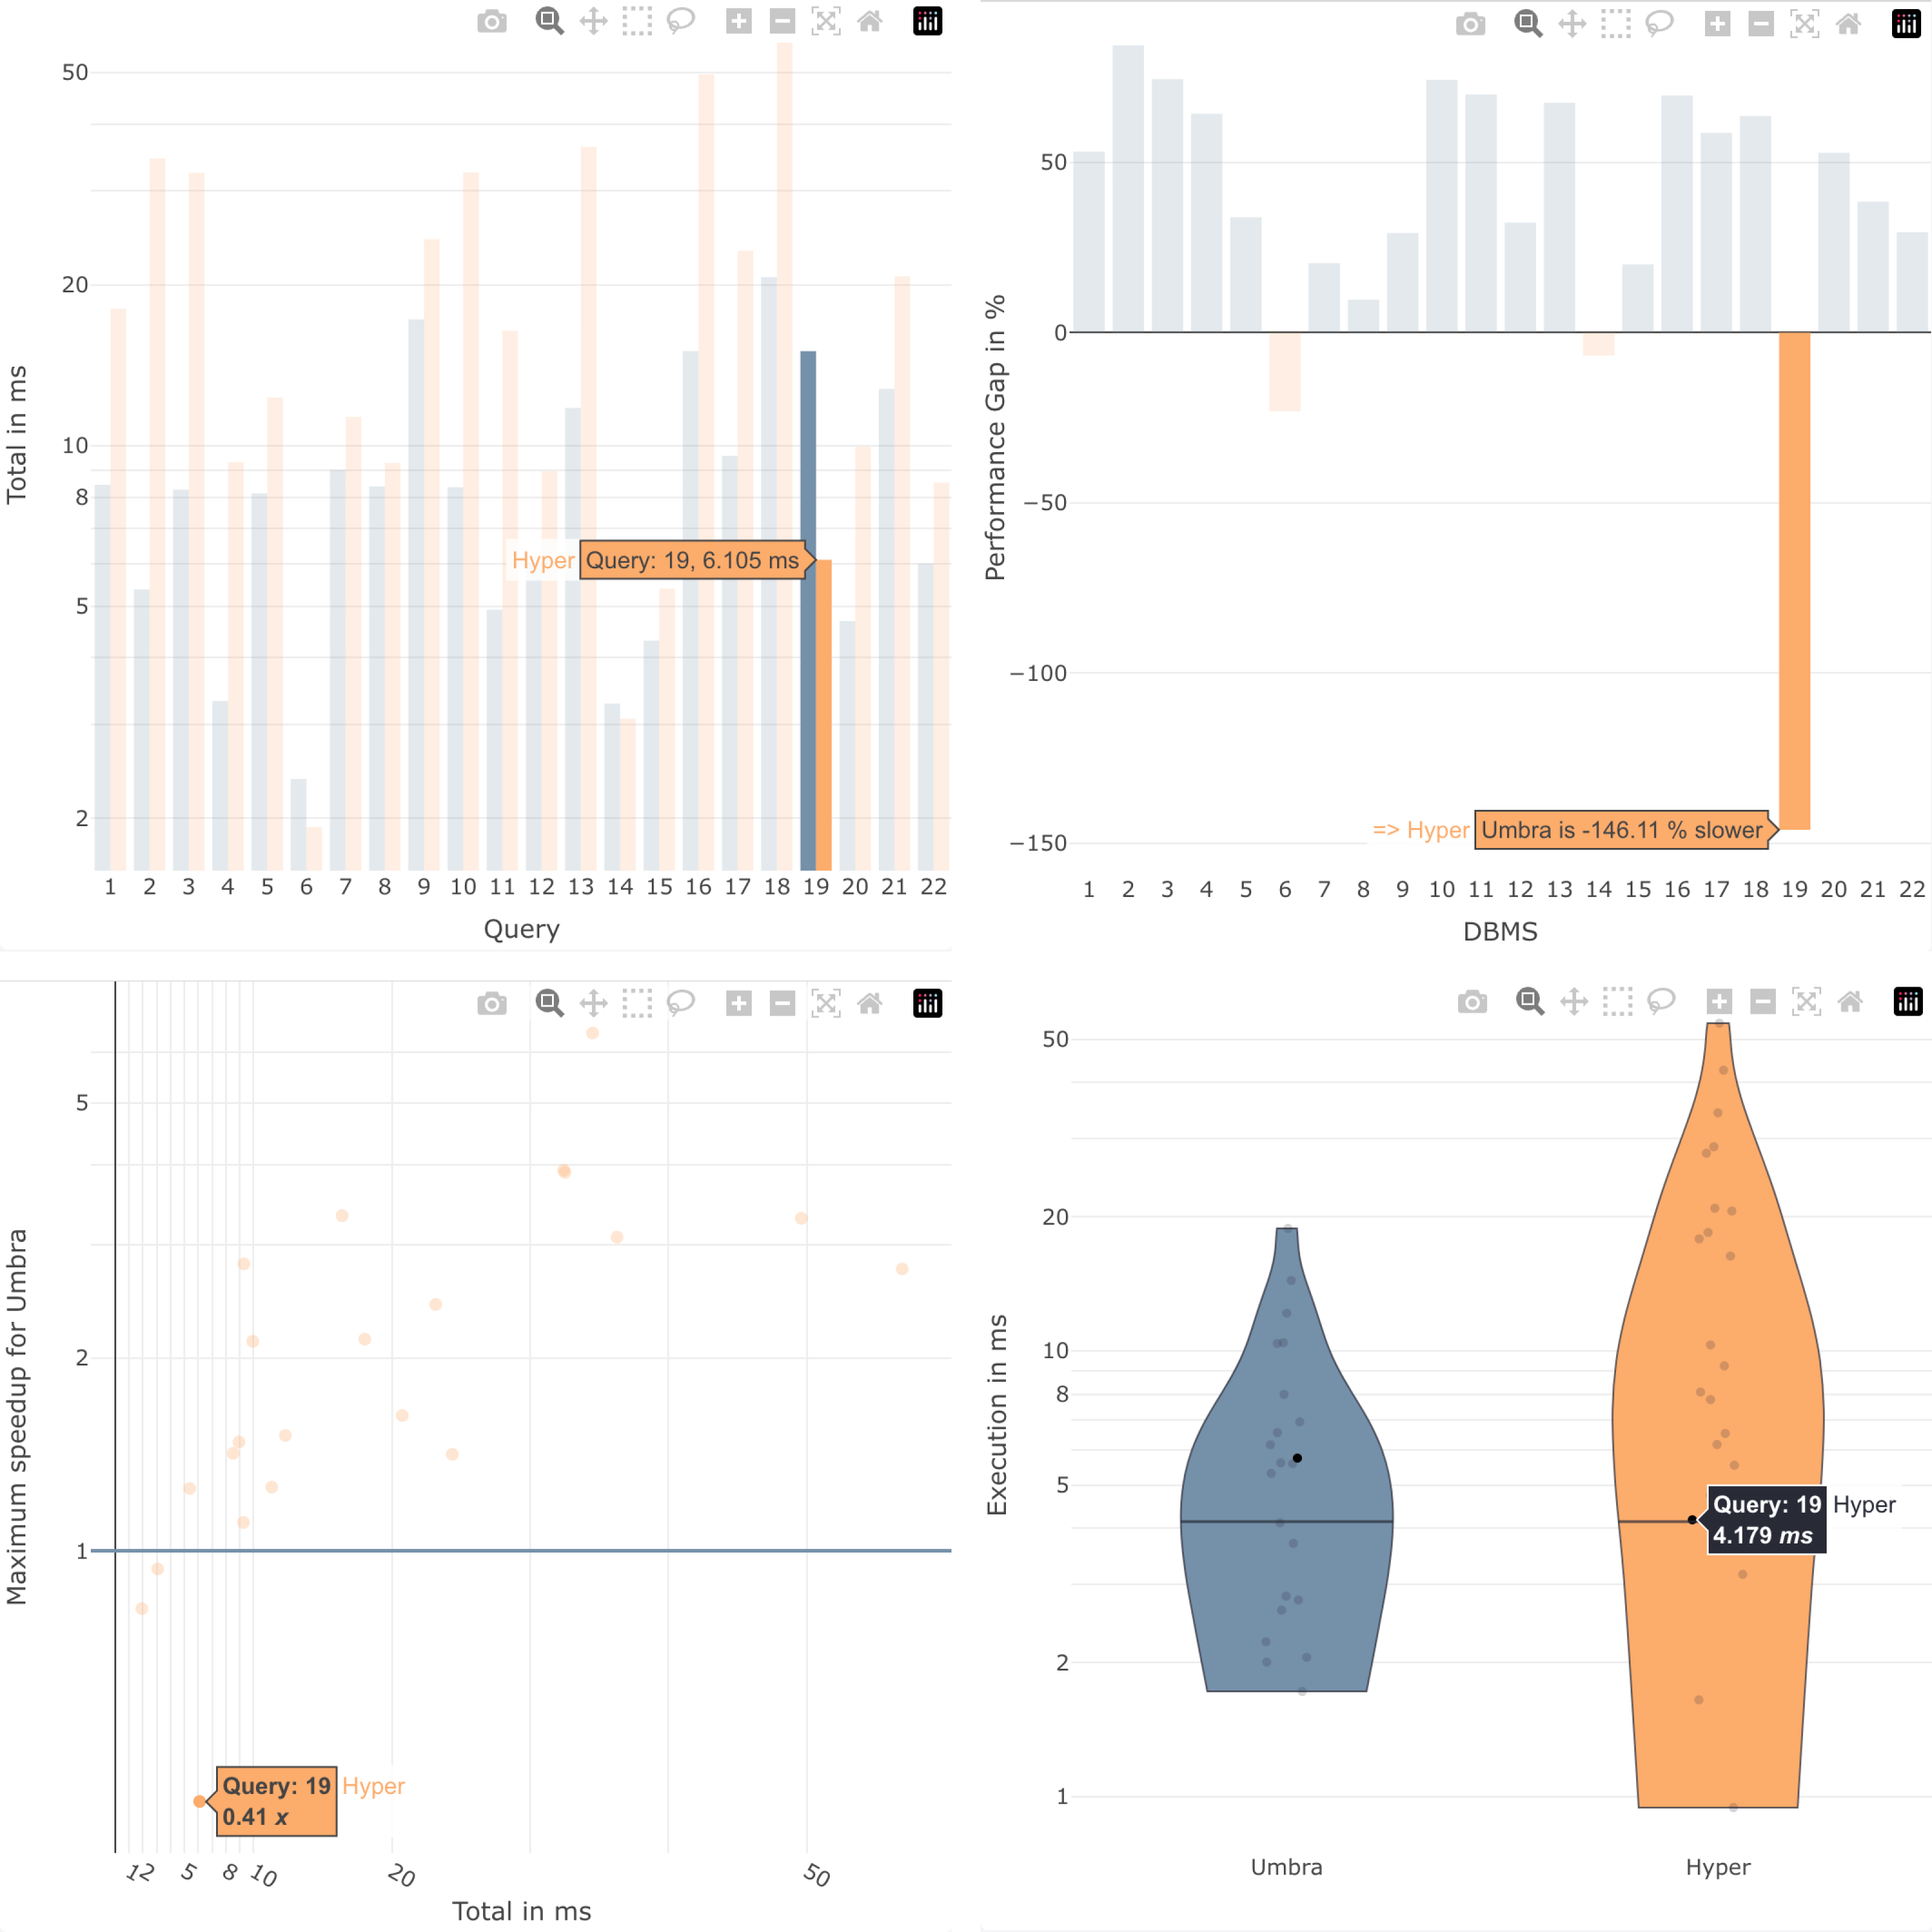
\includegraphics[width=0.6\linewidth]{figures/hover-group.png}
  \caption{Hovering over a query automatically highlights in a global context the same query in all visualizations which are showcasing single queries. These visualizations include violin plots, scatter plots, and bar charts when one bar represents a single query.}
  \label{fig:hover-group}
\end{figure}

Hovering over data points in a chart is an indispensable feature, commonly employed to extract more detailed information about a specific data point. In the context of analysing query performances and identifying noteworthy queries within visualizations, the ability to scrutinize a particular query from multiple perspectives becomes crucial.


 In the Benchy Viewer, we've elevated this feature, which is illustrated in Figure~\ref{fig:hover-group}, to a global hover capability within the application.\\
 This means that when a user hovers over a specific query, not only is that query highlighted within the current chart, but the same queries within all other visualizations are also highlighted simultaneously.This synchronization spans various visualizations, including violin plots, scatter plots, and bar charts which represent distinct queries.



\subsubsection{Data Viewer}

In addition to visualizations, the Benchy Viewer features a data table for in-depth inspection of benchmark data. This table presents the imported user data, as exemplified in the excerpt of the data viewer in Figure~\ref{fig:data-viewer}.

\begin{figure}[h]
  \centering
  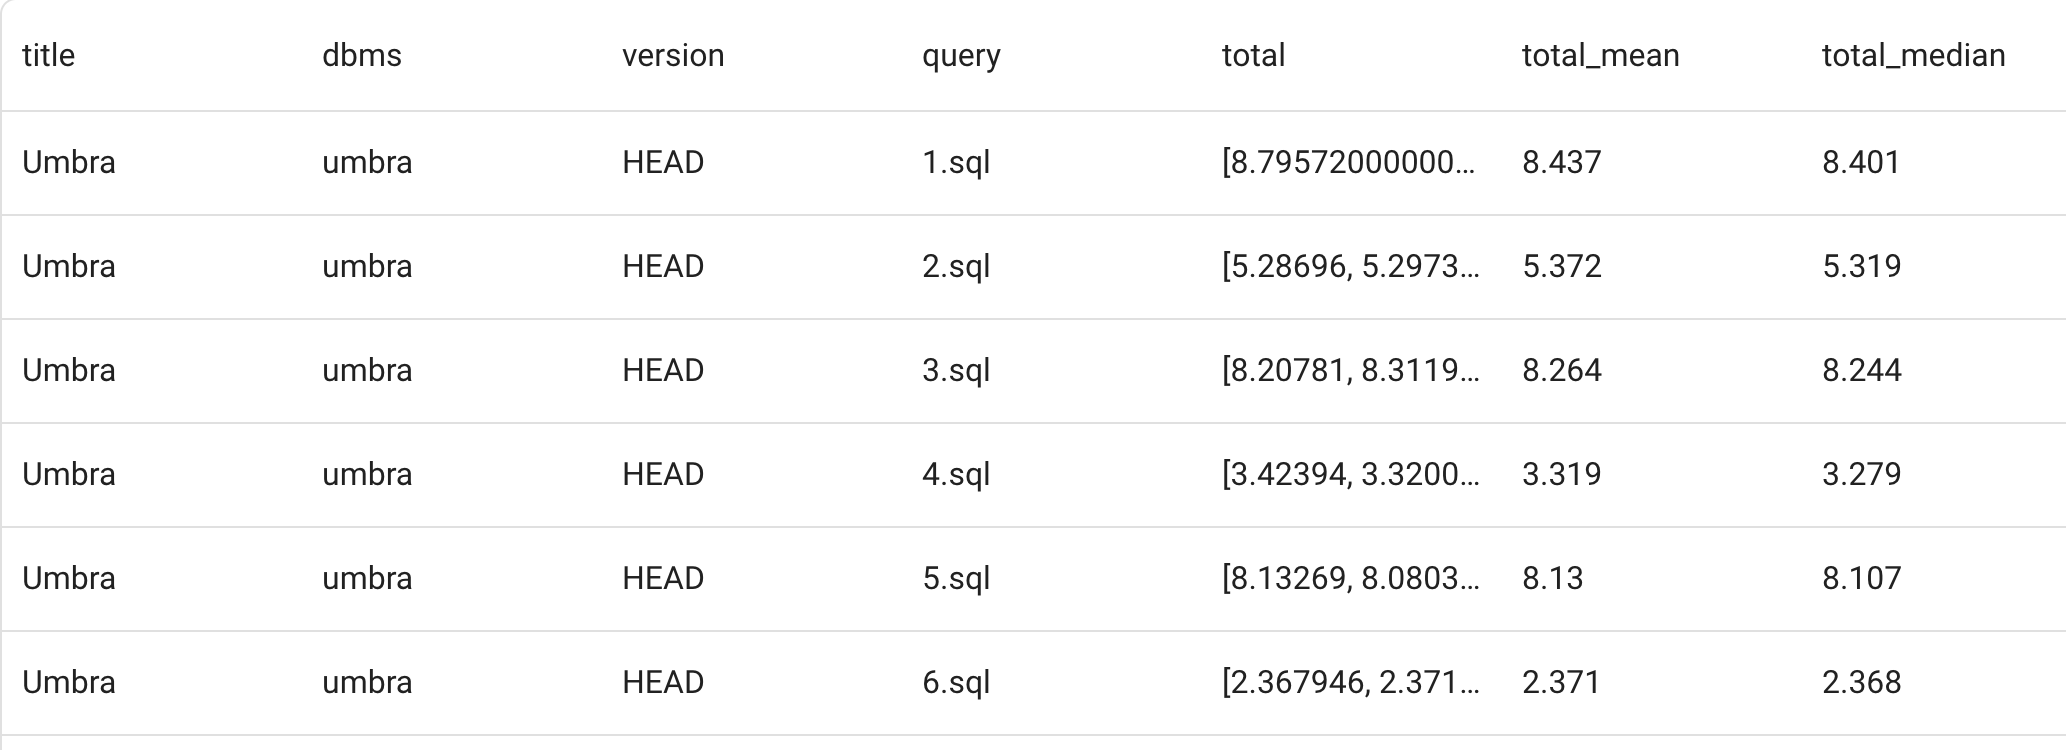
\includegraphics[width=0.9\linewidth]{figures/data-viewer.png}
  \caption{Snapshot of the Data Viewer: Organized rows and columns of benchmark data.}
  \label{fig:data-viewer}
\end{figure}

This view displays the complete data, which is described deeply in section \ref{sec:input-file-structure}.\\
The header contains all properties and metrics of a data row. The data rows below the header represent the data of a query, containing the reference to the database system and the complete benchmark data of this query.\\
The user can scroll vertically and horizontally given the amount of the data rows and the metrics. The header provides some options in a drop-down menu to work with the data sheet, as shown in Figure~\ref{fig:data-viewer-options}. The first option is to sort the table by a chosen data column containing numerical data. The user has the possibility to do this ascending or descending and also reset the sorting. This is useful when the user wants to sort specific data, e.g. the total time in ms.


This view showcases the benchmark data, elaborately described in Section \ref{sec:input-file-structure}. The header encompasses all properties and metrics of a data row. Data rows below the header represent the data of a query, including the reference to the database system and the complete benchmark data for that query.\\
Vertical and horizontal scrolling are enabled to navigate through the extensive data rows and metrics, as the volume of information exceeds the screen's capacity.

\begin{figure}[h]
  \centering
  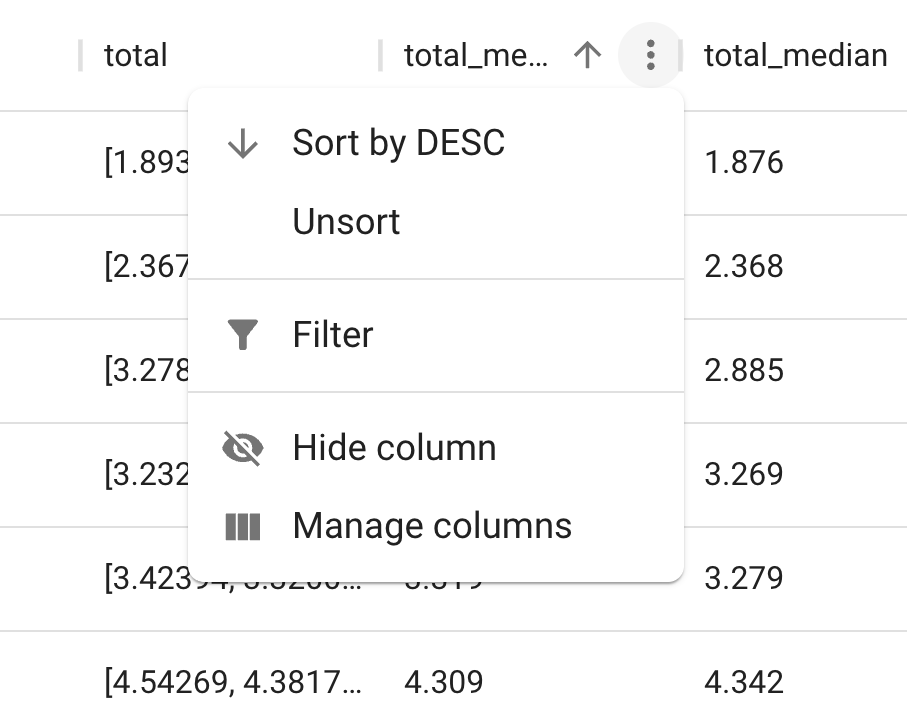
\includegraphics[width=0.4\linewidth]{figures/data-viewer-header-options.png}
  \caption{Column options drop-down offering sorting, filtering, and column visibility functionality.}
  \label{fig:data-viewer-options}
\end{figure}

The header offers various options in a drop-down menu to interact with the data sheet, as depicted in Figure~\ref{fig:data-viewer-options}.

% Sorting
The first option enables sorting the table based on a selected data column with numerical values. Users can choose between ascending or descending order, and there's an option to reset the sorting. This functionality is particularly useful when organizing specific data, for instance, sorting the table based on total time in milliseconds.

\begin{figure}[h]
  \centering
  \begin{subfigure}[b]{0.4\linewidth}
      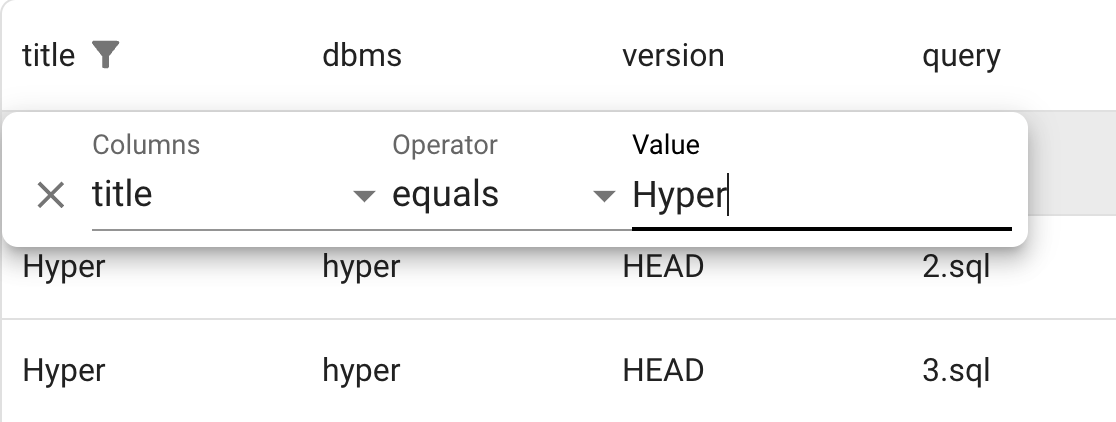
\includegraphics[width=\linewidth]{figures/data-viewer-filter.png}
      \caption{Filter Menu.}
      \label{fig:data-viewer-filter}
  \end{subfigure}
  \hspace{1cm} % Adjust the horizontal space between the figures
  \begin{subfigure}[b]{0.4\linewidth}
      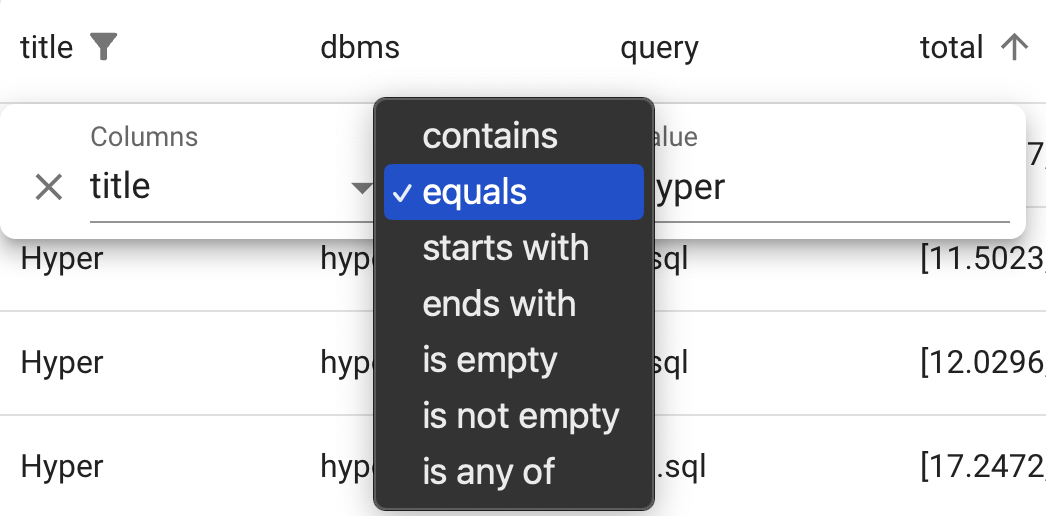
\includegraphics[width=\linewidth]{figures/data-viewer-filter-operator.png}
      \caption{The list of available operators.}
      \label{fig:data-viewer-filter-operator}
  \end{subfigure}
  \caption{Filter menu allows data sheet filtering by column, operator, and value.}
  \label{fig:combined-figures}
\end{figure}

% Filter
The filter option, as shown in Figure~\ref{fig:data-viewer-filter}, provides a tool for refining the displayed data in the table. Users can easily narrow down their focus by selecting a specific column, an operator, and a value. This allows for targeted exploration of the data, such as isolating rows related to a particular database management system, as demonstrated in Figure~\ref{fig:data-viewer-filter-operator}. This filtering capability enhances the user's ability to extract meaningful insights from the benchmark data.


% Manage Columns

\begin{figure}[h]
  \centering
  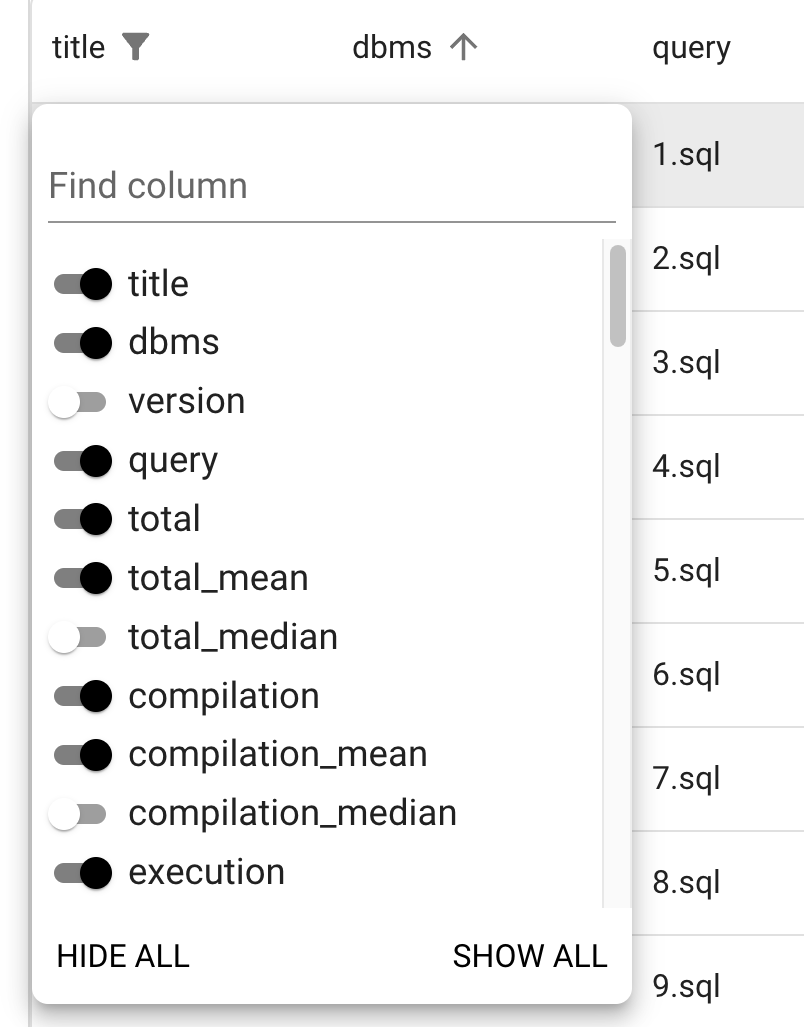
\includegraphics[width=0.35\linewidth]{figures/data-viewer-manage-columns.png}
  \caption{Column Manager: Easily control column visibility in the data sheet for a tailored view.}
  \label{fig:data-viewer-manage-columns}
\end{figure}

When dealing with extensive datasets, the Benchy Viewer ensures flexibility and ease of use by allowing users to tailor their view. Through the 'Manage columns' feature, accessed via the drop-down menu, users can not only hide columns but also gain a holistic overview of active columns. 

Figure~\ref{fig:data-viewer-manage-columns} showcases this functionality, providing users with the ability to effortlessly activate or deactivate columns, conduct quick searches, and streamline their view by hiding or showing all columns at once. This empowers users to focus on the specific data points relevant to their analysis, enhancing the efficiency of the benchmark data exploration process.




\subsection{Query Analytics: Comparative Examination and Comprehensive Benchmark Insight }\label{sec:query-analytics}

One of the primary functions of the Benchy Viewer is to conduct a comparative analysis of the performance across various database systems. The application offers a range of tools for this purpose. In addition to presenting diverse charts and plots for analyzing query data from various angles, the Benchy Viewer allows users to inspect the query plan of a selected query in a comparative manner. To initiate this process, users need to choose the particular query and the involved database systems.

\subsubsection{Preparation for In-Depth Analysis}

In the analytical process of identifying and inspecting a noteworthy query, it is beneficial to refine the information for a more precise and clear understanding.\\
The Benchy Viewer features an interactive legend that not only provides information about group colors but also offers the ability to enable or disable all query visualizations of a system throughout the entire application.

\begin{figure}[h]
  \centering
  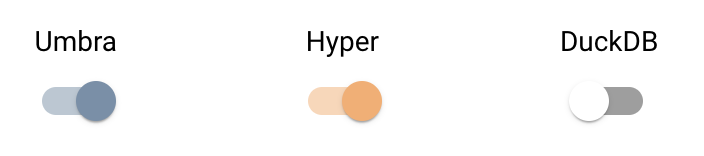
\includegraphics[width=0.4\linewidth]{figures/legend-activate-deactivate.png}
  \caption{Interactive legend with the functionality to activate or deactivate database systems.}
  \label{fig:legend-activate-deactivate}
\end{figure}

This is particularly valuable when a significant query is identified, and a comparison between two systems is of interest, while there are other less relevant systems in the data that may clutter the visualizations. In such cases, users can utilize the interactive header, illustrated in Figure~\ref{fig:legend-activate-deactivate}, to streamline their view and prioritize the visualizations based on current needs.

% Select Queries
In the course of analysing benchmark data and identifying noteworthy queries, a deeper inspection of these queries becomes essential. The Benchy Viewer incorporates a versatile hover feature, as introduced in Section \ref{sec:hover-feature}, providing a multi-perspective view of a specific query by highlighting it across various visualizations simultaneously.

\begin{figure}[h]
  \centering
  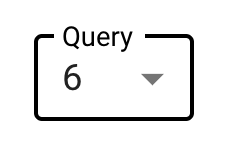
\includegraphics[width=0.15\linewidth]{figures/select-query.png}
  \caption{Drop-down for selecting a specific query for deeper inspection.}
  \label{fig:select-query}
\end{figure}

Similar to this functionality, the Benchy Viewer provides the option to directly select a specific query. This can be accomplished through various means, such as using a drop-down menu, as illustrated in Figure~\ref{fig:select-query}, or by clicking on a specific query data point within a visualization (e.g., clicking on a bar in a bar chart or a data point in a scatter plot).


Selecting a query will also result in highlighting the query in all visualizations, similar to the universal hover feature, also depicted in the Figure~\ref{fig:hover-group}. So, it is possible to highlight two distinct queries at once, the selected query and the hovered query, which enables a comparison between two queries using multiple perspectives. 

Choosing a specific query results in its highlighting across all visualizations, similar to the universal hover feature demonstrated in Figure~\ref{fig:hover-group}. This enables users to concurrently emphasize two separate queries, the chosen query and a hovered one, enabling a comparative analysis from various angles.

\subsubsection{Comprehensive Query Insights}

% Query Plan
In the analysis workflow facilitated by the Benchy Viewer, once a significant query has been identified for more in-depth examination, the subsequent step involves selecting this particular query and transitioning to the Query Plan View. In this phase, users gain the ability to meticulously inspect the query plan associated with the chosen query for each database system under consideration.

The interactive legend, depicted in Figure~\ref{fig:legend-activate-deactivate}, maintains its presence in this view, allowing users to seamlessly activate or deactivate the display of query plans corresponding to specific database systems.

For clarity and comparative analysis, all activated query plans are rendered in a unified visualization. Each query plan is presented in its designated system color. This representation is exemplified in Figure~\ref{fig:query-plan-basic}, where the various query plans are harmoniously displayed for comprehensive comparative scrutiny. This visual approach not only streamlines the analysis process but also contributes to a more intuitive understanding of the comparative performance of queries across different database systems.

\begin{figure}[h]
  \centering
  \begin{subfigure}[b]{0.5\linewidth}
    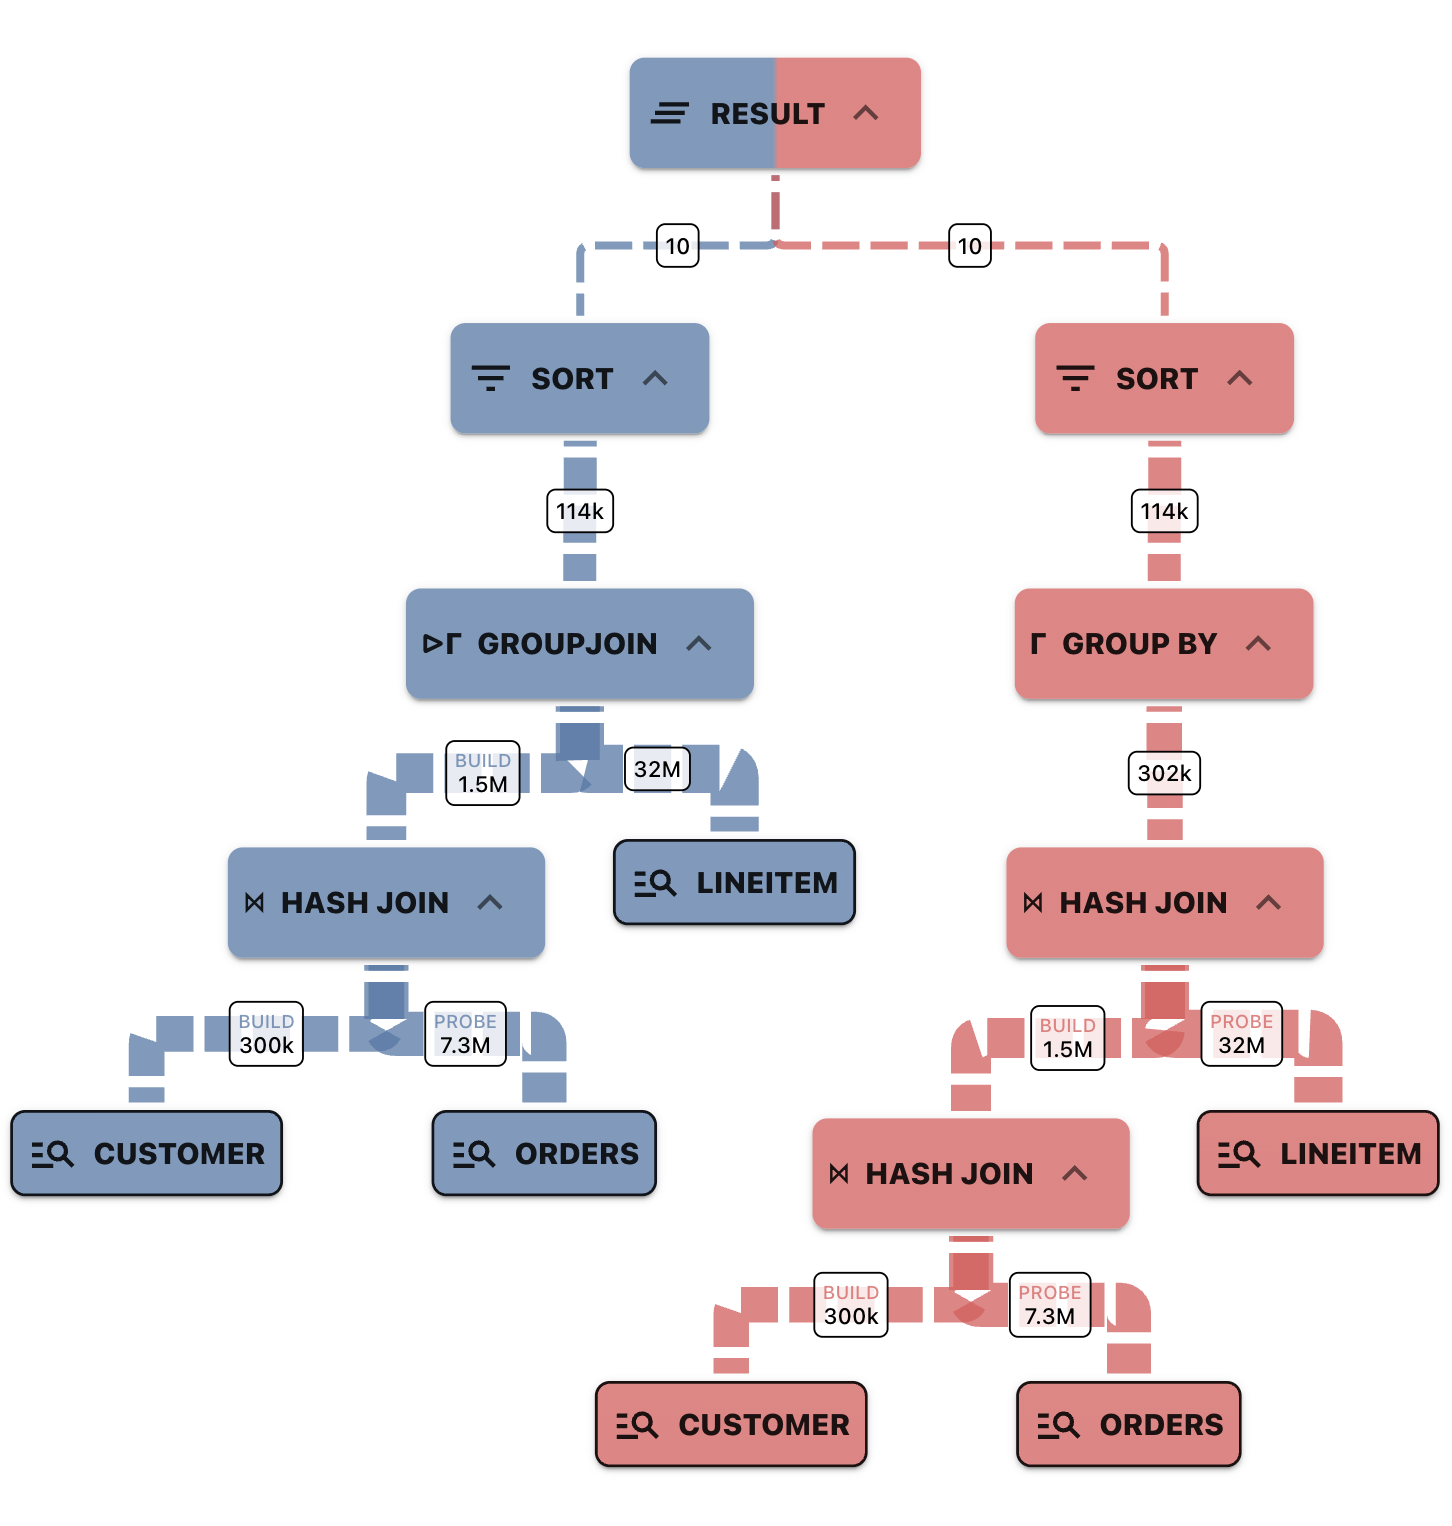
\includegraphics[width=\linewidth]{figures/query-plan-slim.png}
    \caption{Query plan view comparing the query plan of a specific query between two database systems.}
      \label{fig:query-plan-basic}
  \end{subfigure}
  \hspace{1cm} % Adjust the horizontal space between the figures
  \begin{subfigure}[b]{0.35\linewidth}
      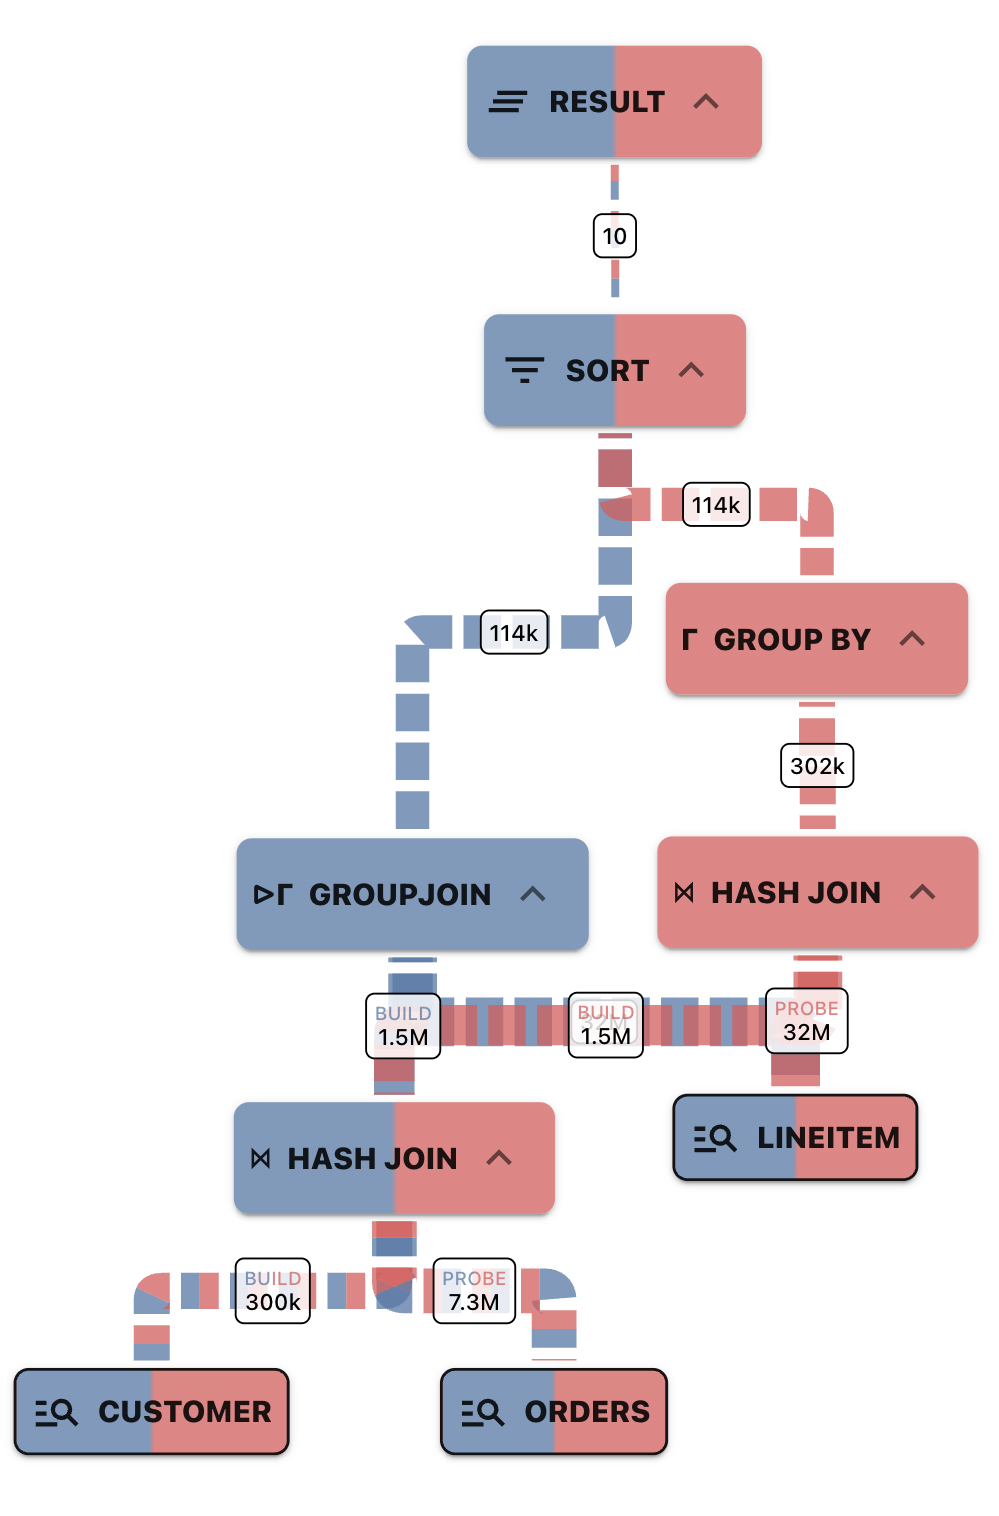
\includegraphics[width=\linewidth]{figures/query-plan-combined-slim.png}
      \caption{Query plan view comparing the query plan of a specific query between two database systems.}
      \label{fig:query-plan-combined}
  \end{subfigure}
  \caption{Query plan comparison between different database systems.}
  \label{fig:query-plan}
\end{figure}


% Funktionen des Query-Plans
The query plan feature is equipped with many tools designed to facilitate a thorough inspection of query plans.
% Combine Trees
A central capability is the merging of all activated query plans using a specified strategy, using the slider illustrated in Figure~\ref{fig:query-plan-slider}. This merging process, exemplified in Figure~\ref{fig:query-plan-combined}, involves summarizing identical subtrees across different plans. Such merging proves invaluable for inspecting divergences in inspected queries, as varying query plan structures are more clearly visualised. For an in-depth exploration of merging strategies, please refer to Section \ref{sec:semantic-diff-integration}.


\begin{figure}[h]
  \centering
  
\includegraphics[width=0.25\linewidth]{figures/query-plan-slider.png}
  \caption{Selection of the query plan merging strategy in the form of a slider.}
  \label{fig:query-plan-slider}
\end{figure}

% Hide Subtree
For extensive query plans, it's beneficial to conceal subtrees that are presently less relevant. This action reduces the overall size of the query plan, emphasizing the more pertinent sections. Users can employ this functionality for any node, as illustrated in Figure~\ref{fig:query-plan-hide-subtree}.

\begin{figure}[h]
  \centering
  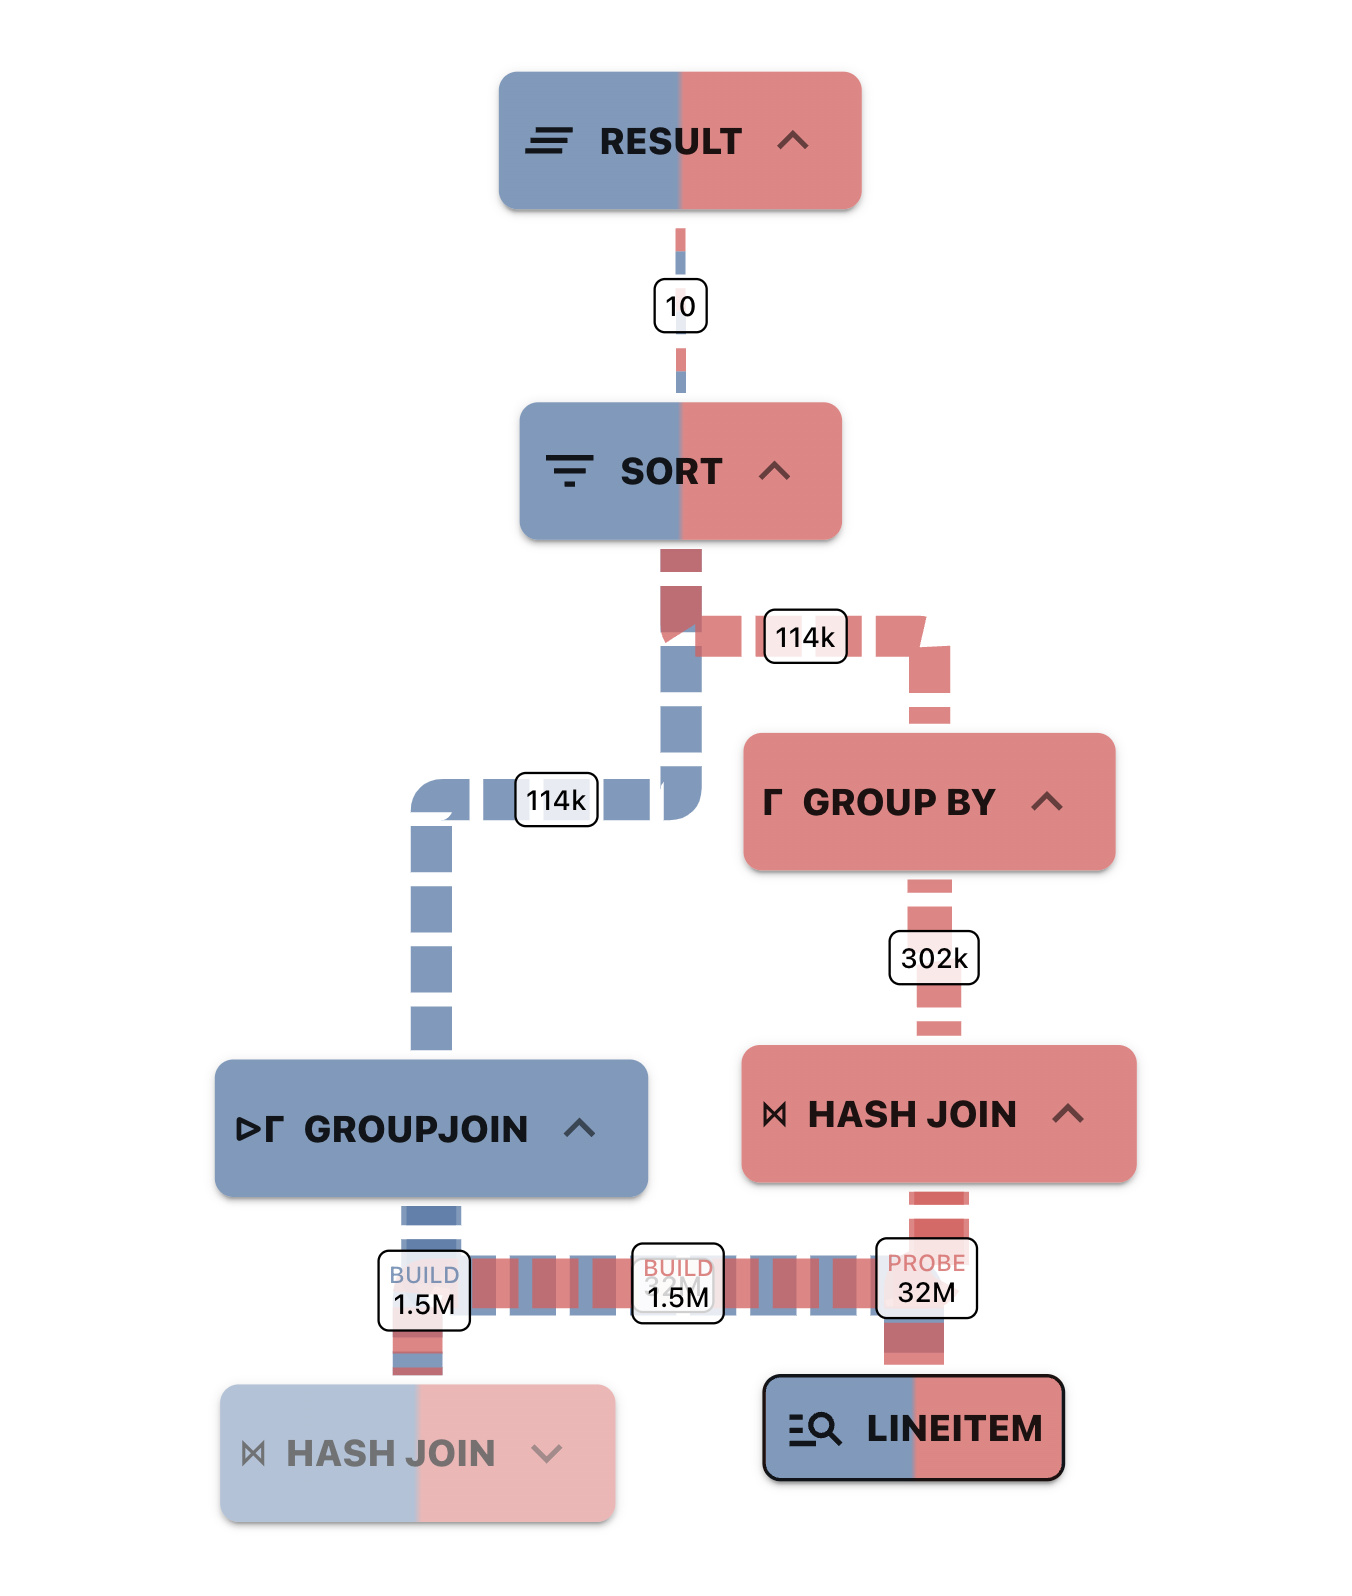
\includegraphics[width=0.35\linewidth]{figures/query-plan-hide-subtree.png}
  \caption{Query plan with a hidden subtree in the bottom left corner.}
  \label{fig:query-plan-hide-subtree}
\end{figure}

% Map
When dealing with extensive query plans, having a tool to comprehend the entire canvas is essential. To facilitate this, a map, as shown in Figure~\ref{fig:query-plan-map}, is included in the bottom right corner of the query plan view. This map provides an overview of the query plans using simplified visual representations of the nodes. Furthermore, it indicates the current location within the complete layout of the query plan, aiding in orientation.

\begin{figure}[h]
  \centering
  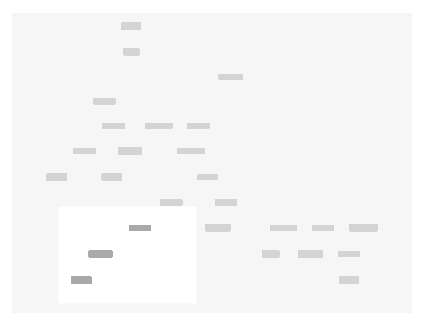
\includegraphics[width=0.25\linewidth]{figures/query-plan-map.png}
  \caption{Map of the query plan showing the current location and the tree in a simplified version.}
  \label{fig:query-plan-map}
\end{figure}

% Node Info, System Representation

The query plan offers supplementary details about nodes. Clicking on a node opens a concise overview, as depicted in Figure~\ref{fig:query-plan-node-info-a}, displaying information about the operator, its type, estimated cardinality, and exact cardinality.\\
In scenarios where multiple databases are activated, and a merged node is selected, the information view shows details for all systems being merged within that node, as illustrated in Figure~\ref{fig:query-plan-node-info-combined}.

\begin{figure}[h]
  \centering
  \begin{subfigure}[b]{0.4\linewidth}
    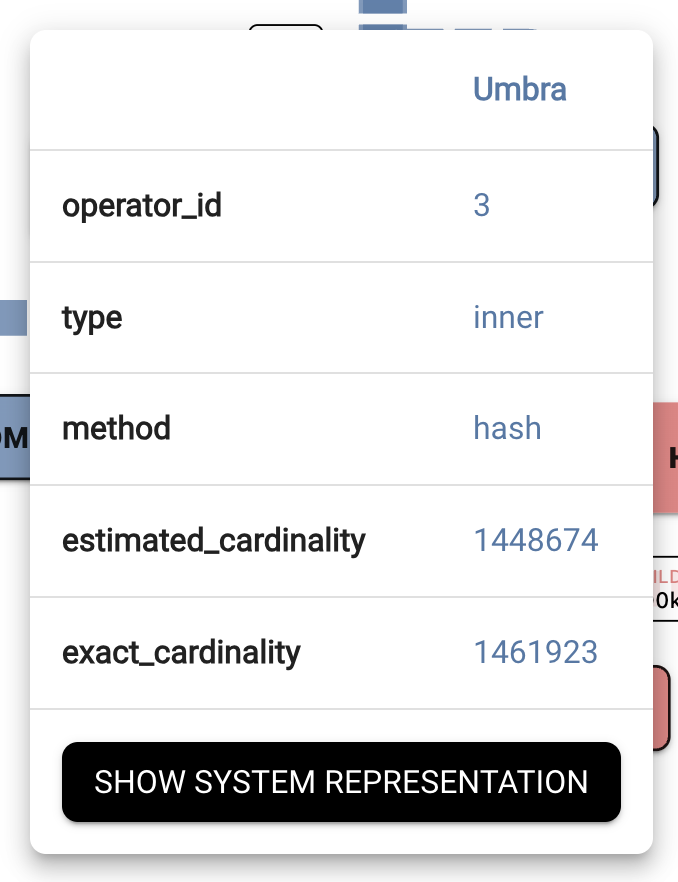
\includegraphics[width=0.7\linewidth]{figures/query-plan-node-info.png}
    \caption{Node information window.}
      \label{fig:query-plan-node-info-a}
  \end{subfigure}
  \hspace{1cm} % Adjust the horizontal space between the figures
  \begin{subfigure}[b]{0.4\linewidth}
      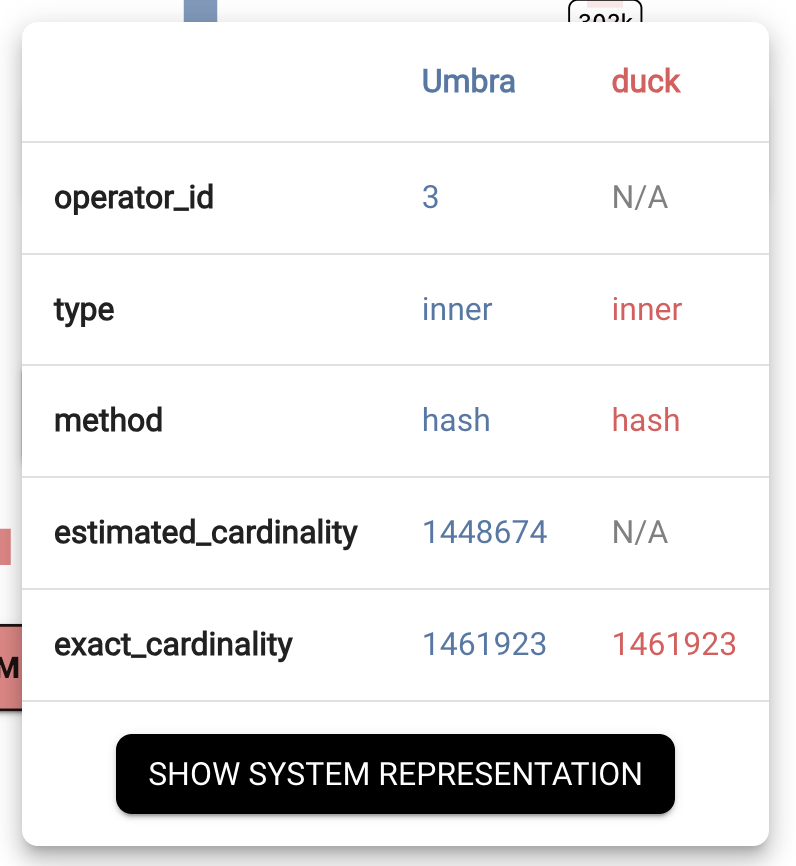
\includegraphics[width=0.8\linewidth]{figures/query-plan-node-info-combined.png}
      \caption{Node information window of a shared node.}
      \label{fig:query-plan-node-info-combined}
  \end{subfigure}
  \caption{Node information window of the selected node.}
  \label{fig:query-plan-node-info}
\end{figure}

The information window also allows displaying the system representation. As an overlay, similar to Figure~\ref{fig:query-plan-system-representation}, the system representation appears in the style of a simple code editor, presenting information in a code-like format. Line numbers are displayed on the left, and an overview of the file is shown on the right.

\begin{figure}[h]
  \centering
  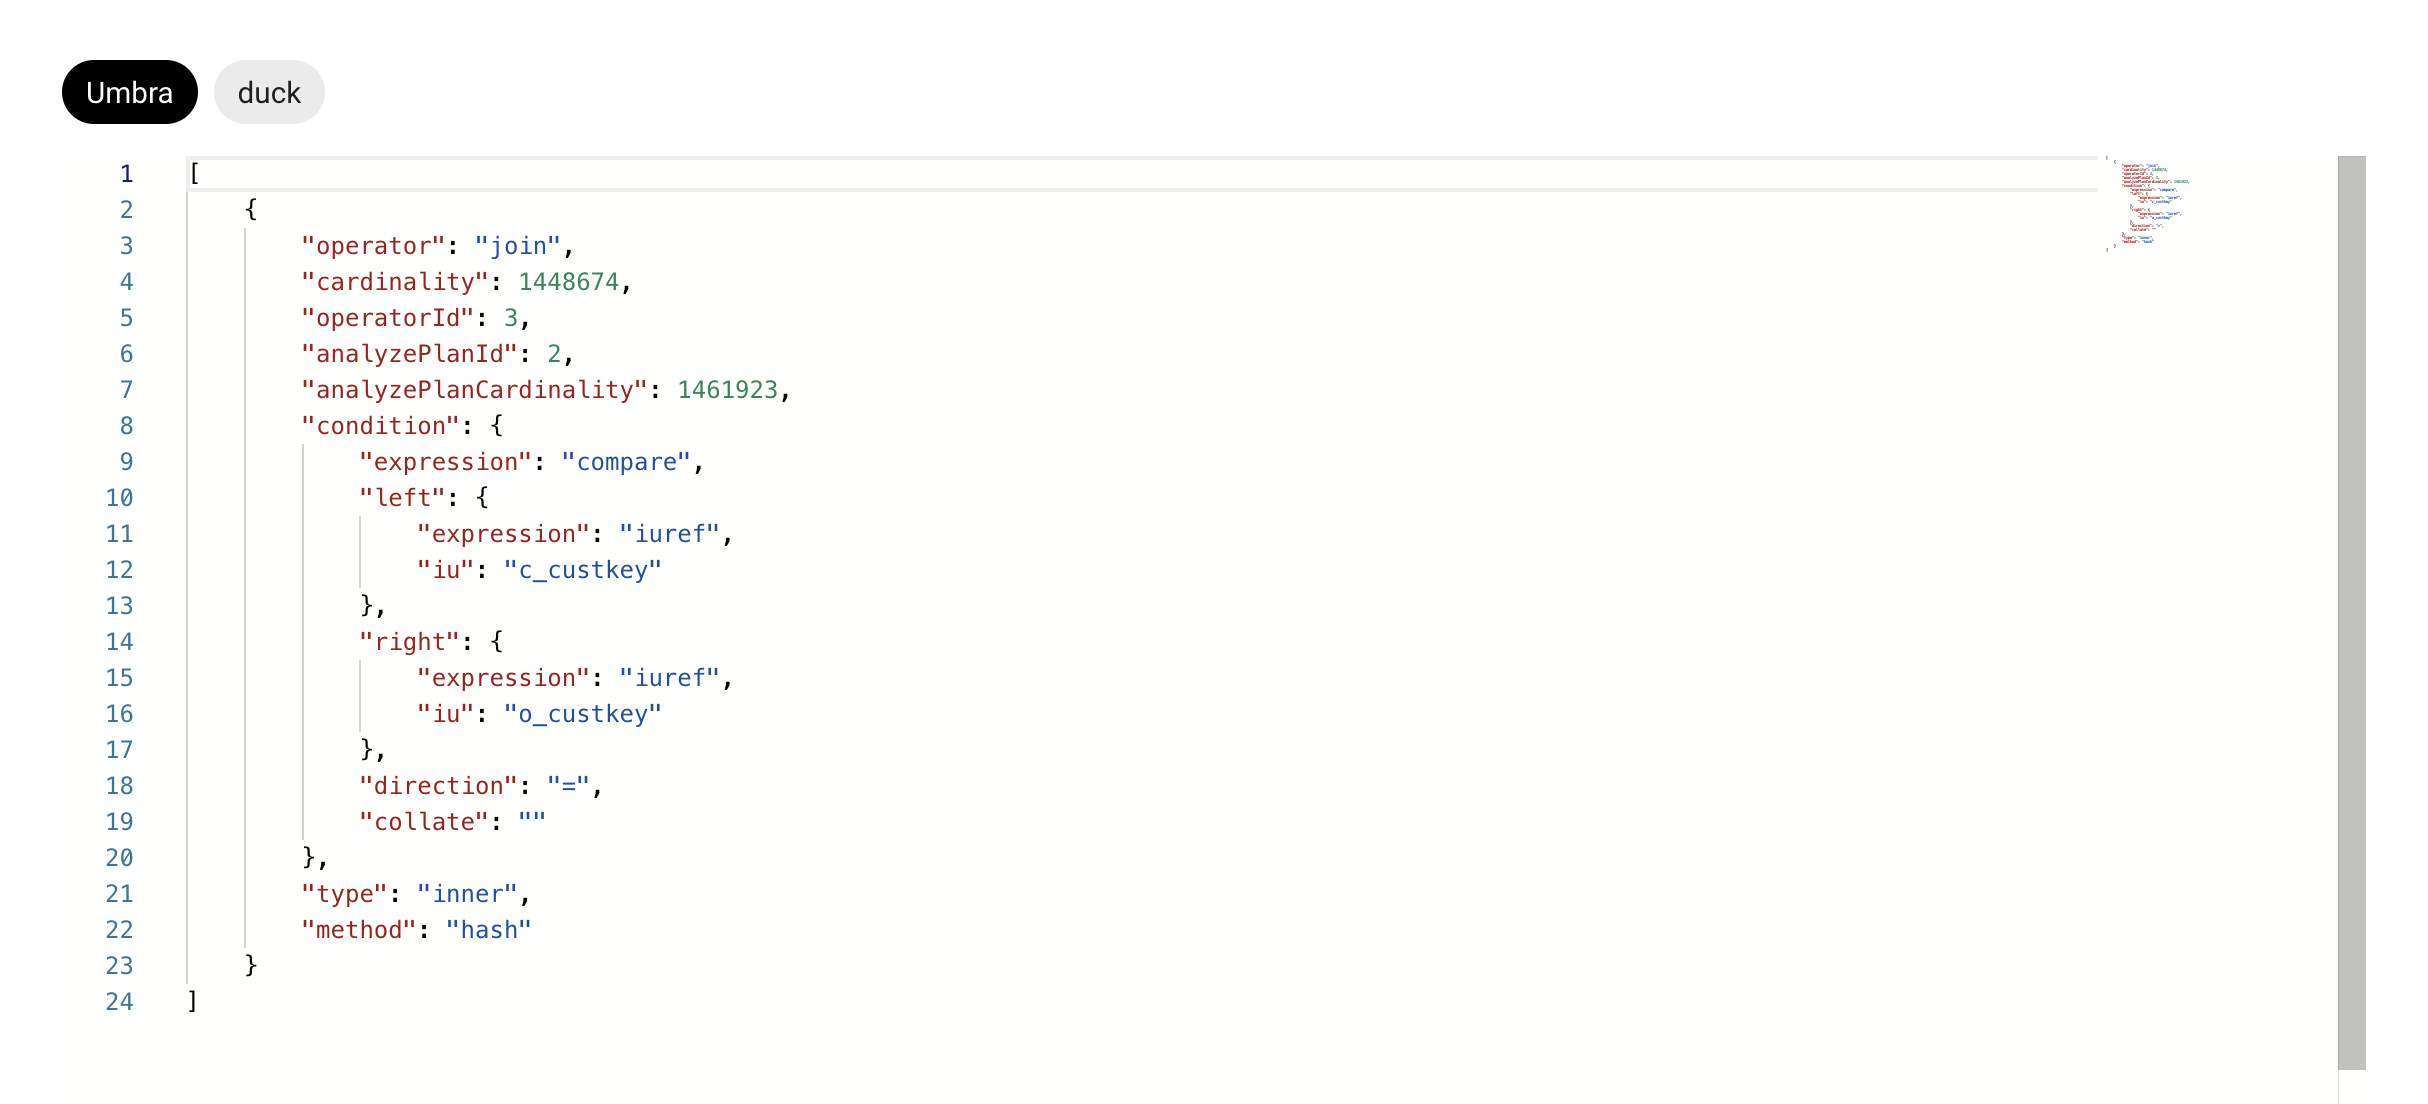
\includegraphics[width=0.8\linewidth]{figures/query-plan-node-system-representation-combined.png}
  \caption{Query plan system representaion of a node.}
  \label{fig:query-plan-system-representation}
\end{figure}

At the top, the user can choose the database system for which the system representation should be displayed in the case of a merged node.

All these functionalities are provided by the semantic diff tool \textcolor{red}{ZITAT}. We dive deeper into the integration of the semantic diff tool in the section \ref{sec:semantic-diff-integration}.


\subsection{Flexible Interface Hub}

To offer a well-suited platform for analysing specific performance differences of high complexity, a flexible system is essential for conducting these analytical processes. Such flexibility is crucial for providing tailored solutions to inspect specific aspects of benchmark data.

In this section, we will explore how the Benchy Viewer achieves this functionality, primarily through a drag-and-drop system for visualization elements. This empowers users to select the necessary visualizations and construct a comprehensive overview.

Subsequently, we will delve deeper into the actual visualizations, examining the flexibility of configuring charts and plots to optimize the perspective of performance data within a specific visualization.

\subsubsection{Drag and Drop}
The drag-and-drop system integrated into the Benchy Viewer empowers users to effortlessly rearrange every chart and plot. Beyond the flexibility offered by individual visualization elements, users can strategically organize visualizations within containers. These containers are essentially thematic sections, each represented by a headline. Users have the flexibility to rename these containers, creating dedicated spaces for specific topics and populating them with relevant charts and plots.

\begin{figure}[h]
  \centering
  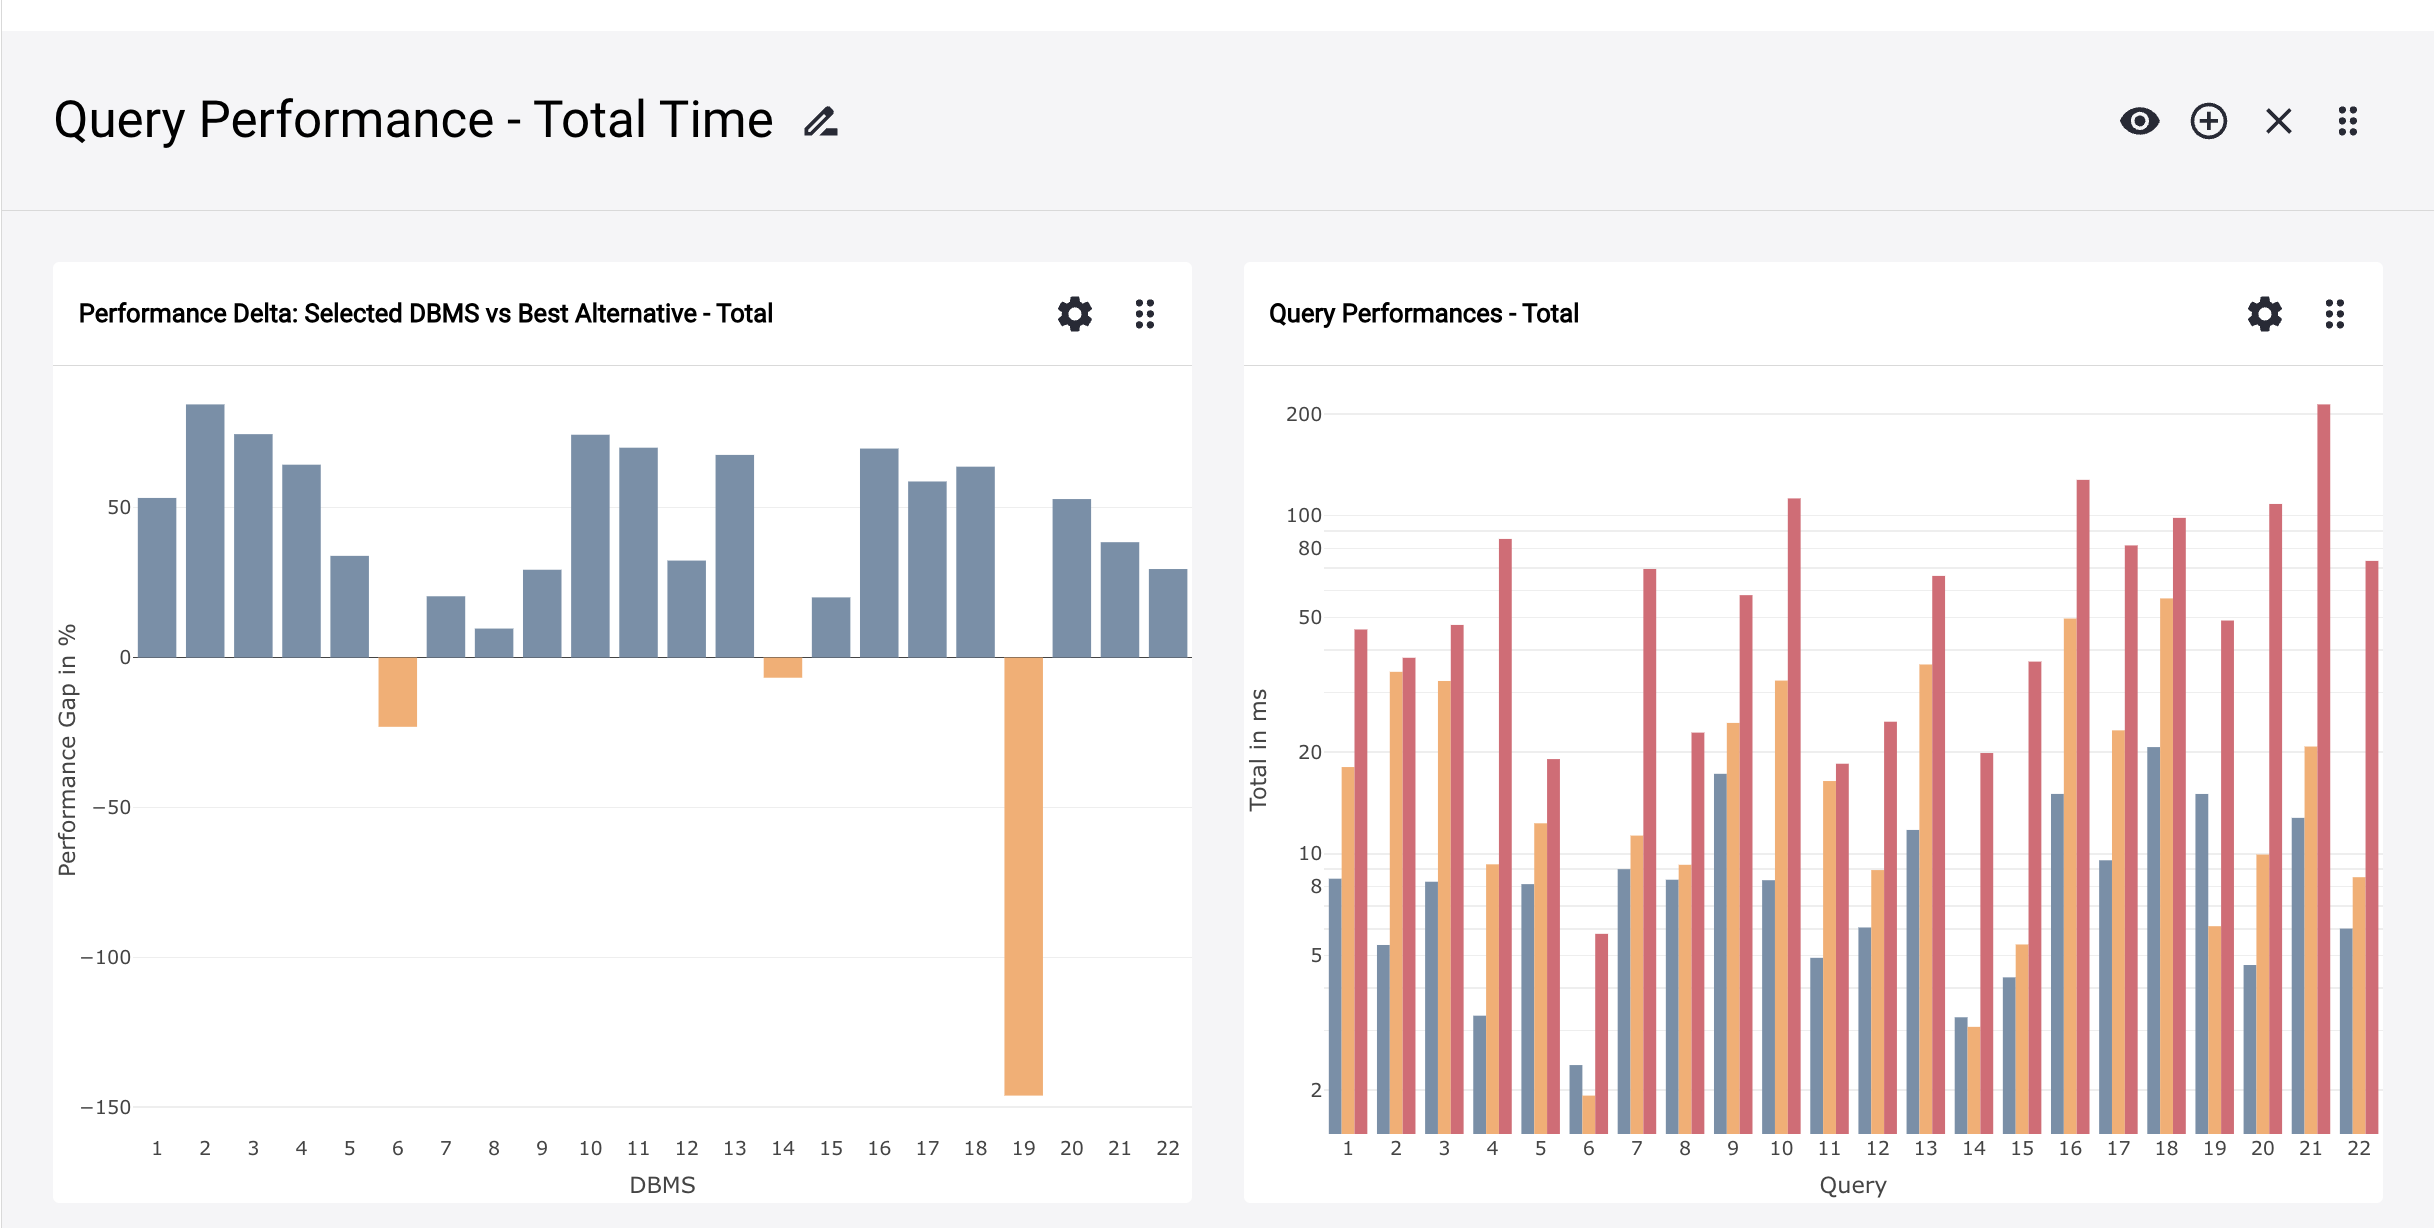
\includegraphics[width=0.8\linewidth]{figures/analytics-drag-and-drop.png}
  \caption{Flexible interface hub through drag and drop feature for visualization elements and their containers.}
  \label{fig:analytics-drag-and-drop}
\end{figure}

The versatility of containers allows them to function as distinct analytical sections, housing visualization elements pertinent to that specific context. Moreover, the dynamic nature of the Benchy Viewer enables users to seamlessly move visualizations between containers, fostering adaptability in organizing and categorizing data. The ability to drag entire containers further enhances this adaptability, enabling users to arrange sections according to their analytical preferences. This dual flexibility, within containers and with container placement, provides users with a robust framework for tailoring their analytical environment to meet the demands of diverse datasets.

\subsubsection{Analytics Sections}

% Rename Section
The top header of a container, as illustrated in Figure~\ref{fig:analytics-drag-and-drop}, serves as a hub for fundamental container functionalities. An intuitive feature allows users to rename a container by clicking on the edit icon situated next to the container's label. This action triggers a dialogue with a straightforward text input, as depicted in Figure~\ref{fig:analytics-section-rename}. Once users input and confirm the new label using the "ok" button, the container's label promptly updates.\\
Users can now efficiently organize and contextualize their analytical elements within appropriately named containers. The ability to swiftly modify container labels enhances the user experience, enabling them to maintain a well-structured and easily navigable analytical workspace.

\begin{figure}[h]
  \centering
  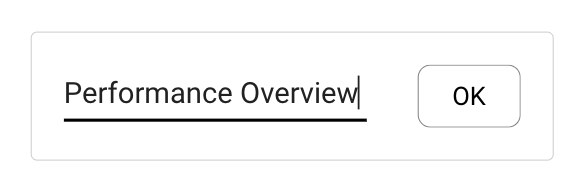
\includegraphics[width=0.25\linewidth]{figures/analytics-section-rename.png}
  \caption{Text input for renaming containers.}
  \label{fig:analytics-section-rename}
\end{figure}

% Add chart
To enrich the content within a container, users can effortlessly incorporate charts and plots using the icon positioned in the right corner of the container's header. This action opens an overlay menu presenting a variety of available plots and charts for inclusion in the container, as showcased in Figure~\ref{fig:analytics-add-chart}. Upon the user's selection of a visualization element, the analytical section promptly updates, seamlessly integrating the chosen element into its content.

\begin{figure}[h]
  \centering
  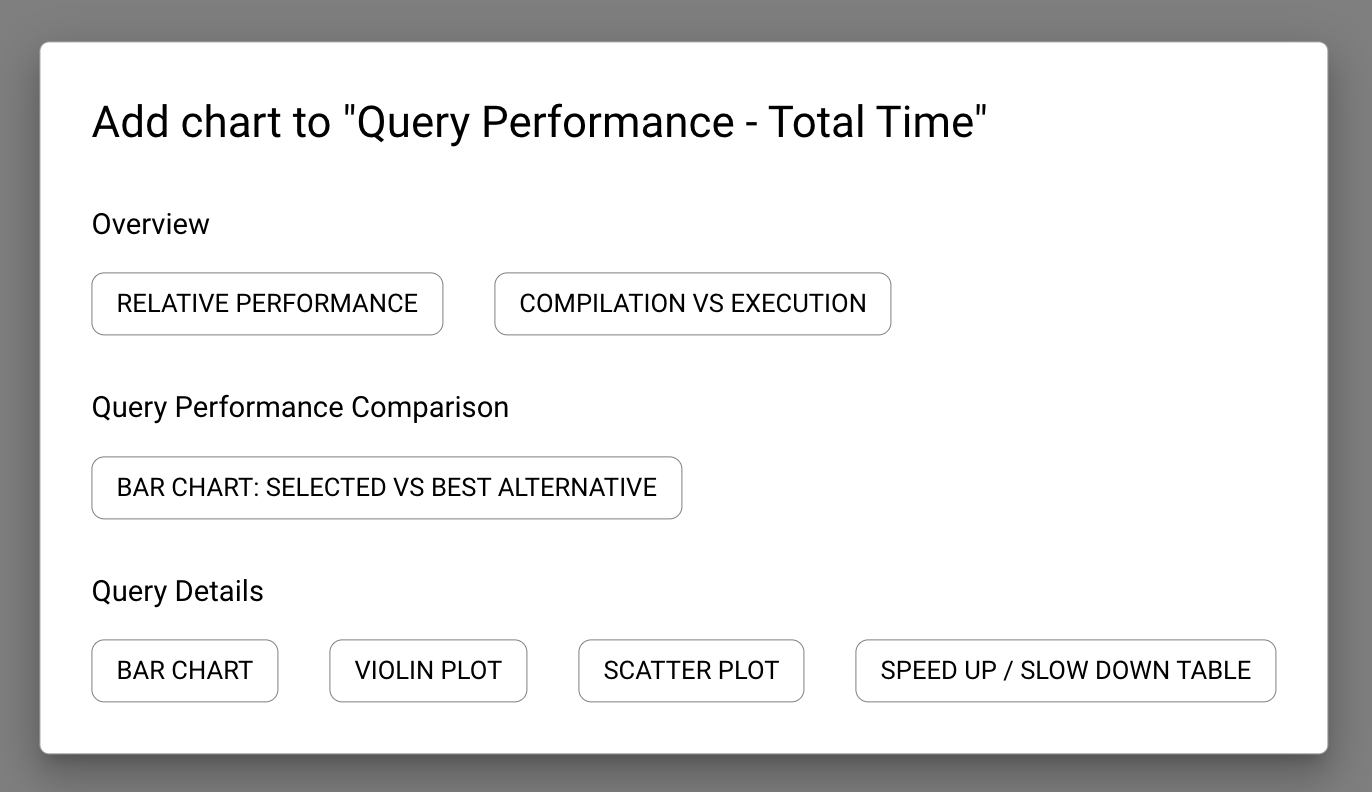
\includegraphics[width=0.6\linewidth]{figures/analytics-add-chart.png}
  \caption{Overlay for adding charts to the current container.}
  \label{fig:analytics-add-chart}
\end{figure}

This intuitive process streamlines the augmentation of analytical sections, allowing users to dynamically enhance their workspace with relevant visualizations. The added charts and plots are instantly ready for utilization, fostering a fluid and responsive analytical environment within the Benchy Viewer.\\
We dive deeper into the utilization and configuration of the charts and plots in \ref{sec:chart-configuration}.


% Set Visibility of containers
Another valuable functionality in the container's header is the visibility toggle. Users can swiftly conceal an analytics section by simply clicking the visibility icon of a container, as illustrated in Figure~\ref{fig:analytics-section-visibility}. This action disables the view of the content, revealing only the header of the container. Users can easily reactivate visibility or access other functionalities.

\begin{figure}[h]
  \centering
  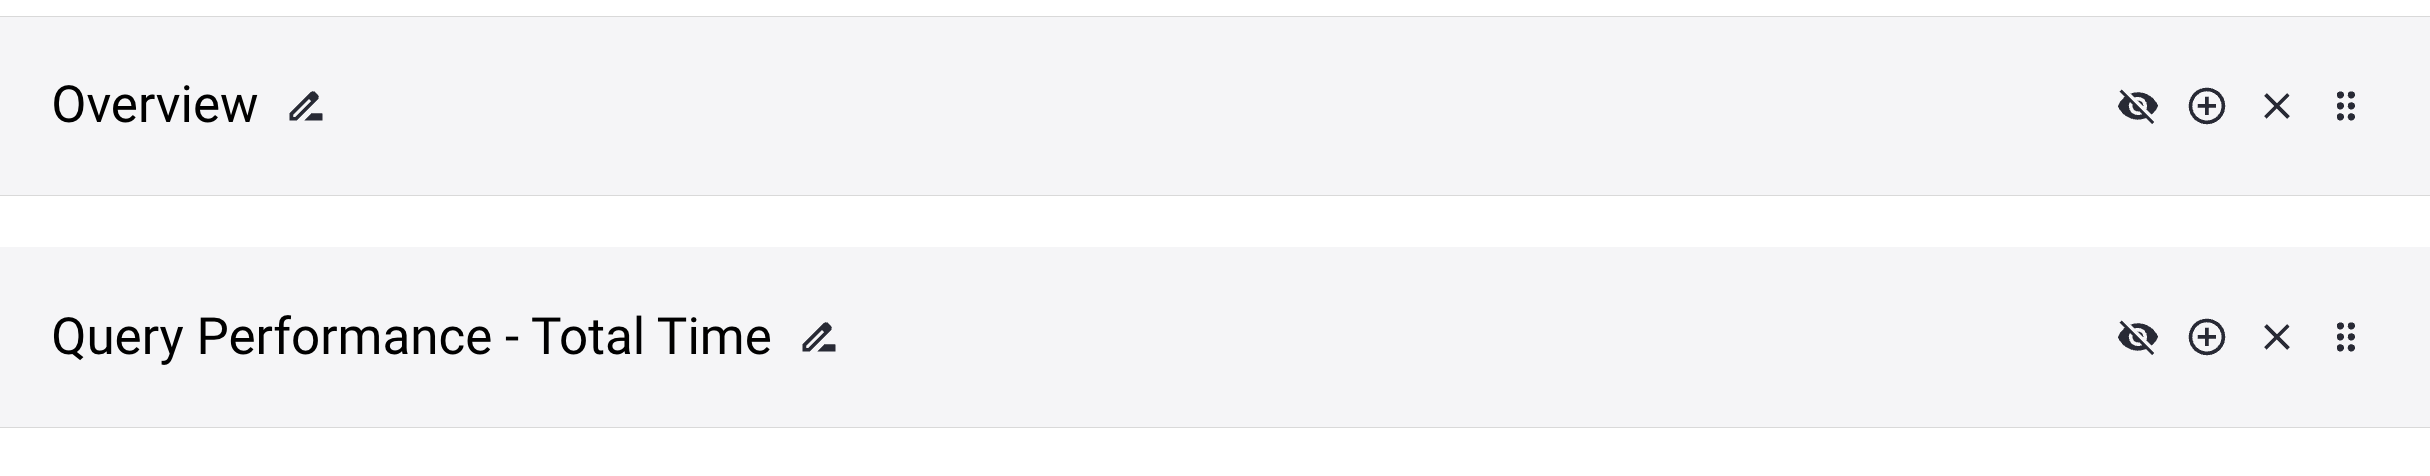
\includegraphics[width=0.8\linewidth]{figures/analytics-section-visibility.png}
  \caption{Visibility property to hide or show a container.}
  \label{fig:analytics-section-visibility}
\end{figure}

The convenience of collapsing containers, coupled with the drag-and-drop feature, enhances overall user comfort and efficiency. This uncomplicated feature significantly enhances clarity and ease of use, especially when managing a substantial number of visualizations and diverse data perspectives.

Initiating the deletion process, another noteworthy feature embedded in the container's header is the delete function. By clicking on the delete icon of a container, users can efficiently remove an analytics section. This action permanently eliminates the container and its content. This straightforward delete function provides a quick and effective way to manage the organizational structure of visualizations.


\subsubsection{Chart Configurations}\label{sec:chart-configuration}

Within the Benchy Viewer, a versatile dashboard serves as a backdrop for seamless interaction with diverse visualizations. Delving into individual visualization elements, the platform prioritizes adaptability, allowing users to tailor charts and plots to their specific requirements.\\
We'll explore the capability to select a metric within a chart, demonstrate the flexibility of switching to a table visualization in the context of maximum speed-up and maximum slow-down, and finally, highlight global chart options.

\begin{figure}[h]
  \centering
  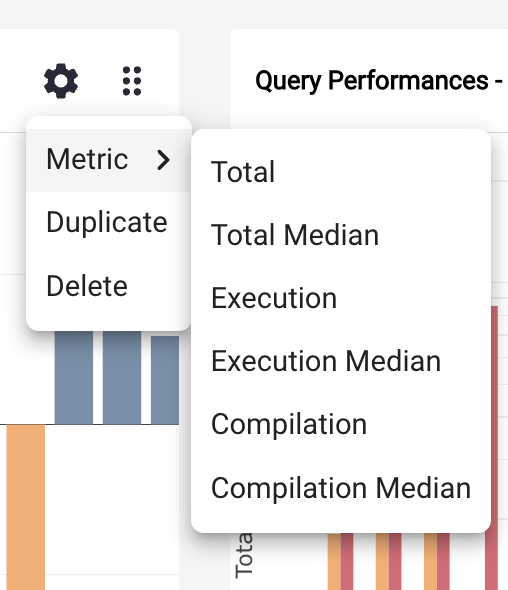
\includegraphics[width=0.35\linewidth]{figures/chart-configuration.png}
  \caption{Drop-down menu of chart options offering to select the visualised metric. Also the delete and duplicate functionality is provided.}
  \label{fig:chart-configuration}
\end{figure}

% - Metrics auswählen
Every visualization element within the drag-and-drop dashboard features a header, as illustrated in Figure~\ref{fig:analytics-drag-and-drop}. Beyond the drag-and-drop functionality, the header hosts an options icon, providing access to various configuration settings, as depicted in Figure~\ref{fig:chart-configuration}.\\
Within the nested drop-down menu, users can seamlessly tailor their selection of metrics to meet specific needs.

Upon selecting a metric, the chart dynamically updates, presenting the new data within the current visualization framework. This rapid and flexible construction of charts enhances the user's ability to gain valuable insights swiftly.

Similarly, users can quickly duplicate a chart for comparative analysis or delete it to streamline the dashboard. The duplicate function allows for the replication of a chart with its current settings, providing an efficient way to explore variations of the same data.\\
Conversely, the delete function promptly removes a chart, contributing to a clutter-free and focused visual workspace. These functionalities collectively empower users to fine-tune their analytical environment for a seamless exploration experience.

% - tabele und scatter: speed-up/ slow-down
In the analytical process of working with the metric pair speed-up and slow-down, seamlessly toggling between maximum speed-up and maximum slow-down is crucial. The Benchy Viewer facilitates this transition through the switch icon integrated into the header of the table visualization, as exemplified in Figure~\ref{fig:chart-configuration-table-switch}.

\begin{figure}[h]
  \centering
  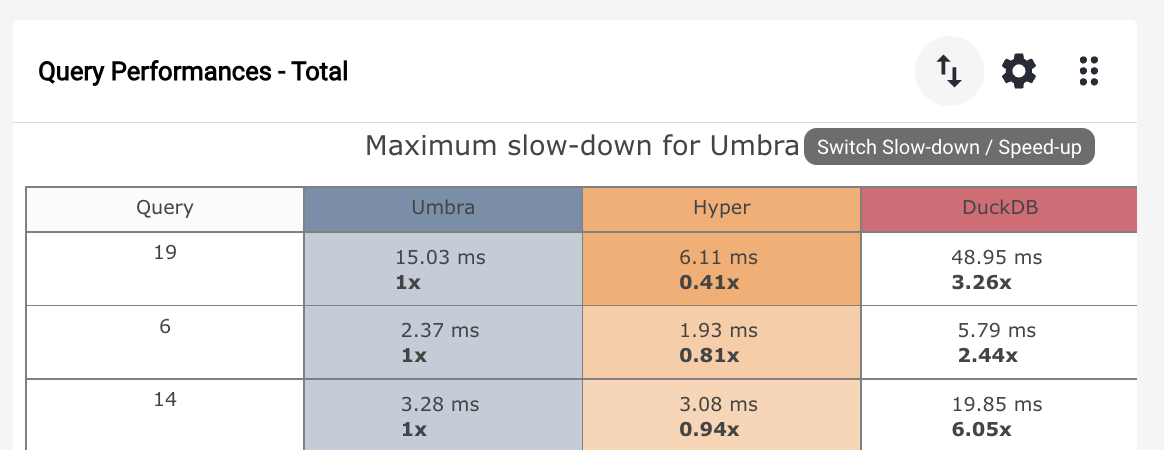
\includegraphics[width=0.8\linewidth]{figures/chart-configuration-table-switch.png}
  \caption{Table visualization provides the functionality to switch between maximum speed-up and maximum slow-down.}
  \label{fig:chart-configuration-table-switch}
\end{figure}

A simple click on the switch icon triggers the table to transition to the alternate mode, dynamically updating its data to reflect the chosen metric. This feature ensures a fluid and efficient exploration of performance data, allowing users to effortlessly switch between speed-up and slow-down perspectives as needed.


% - Scale: Linear/ Log/ Throuput
In addition to the nuanced control over individual visualizations, the Benchy Viewer empowers users with global chart options, allowing users to sculpt the visual landscape to their specific analytical requirements.

One of the noteworthy features is the ability to globally switch the Y-axis type, as depicted in Figure~\ref{fig:chart-configuration-scale}. This flexibility allows users to choose between linear, logarithmic, and throughput representations, offering diverse perspectives on the benchmark data. Whether aiming for a detailed examination of variations in lower values or emphasizing proportional changes, the global Y-axis type switch ensures that the visualizations align with the user's analytical focus.

\begin{figure}[h]
  \centering
  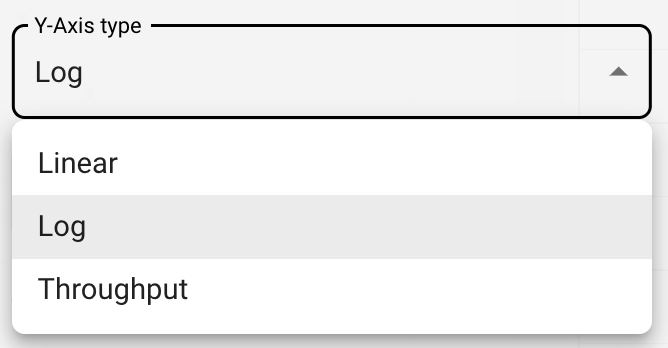
\includegraphics[width=0.3\linewidth]{figures/chart-configuration-scale.png}
  \caption{Drop-down menu of global options offering the selection of the scale type.}
  \label{fig:chart-configuration-scale}
\end{figure}

The linear scale is ideal when a precise examination of small variations in data is paramount. This scale excels in offering a detailed, granular view, particularly advantageous for closely positioned metric values.

\begin{figure}[h]
  \centering
  \begin{subfigure}[b]{0.3\linewidth}
    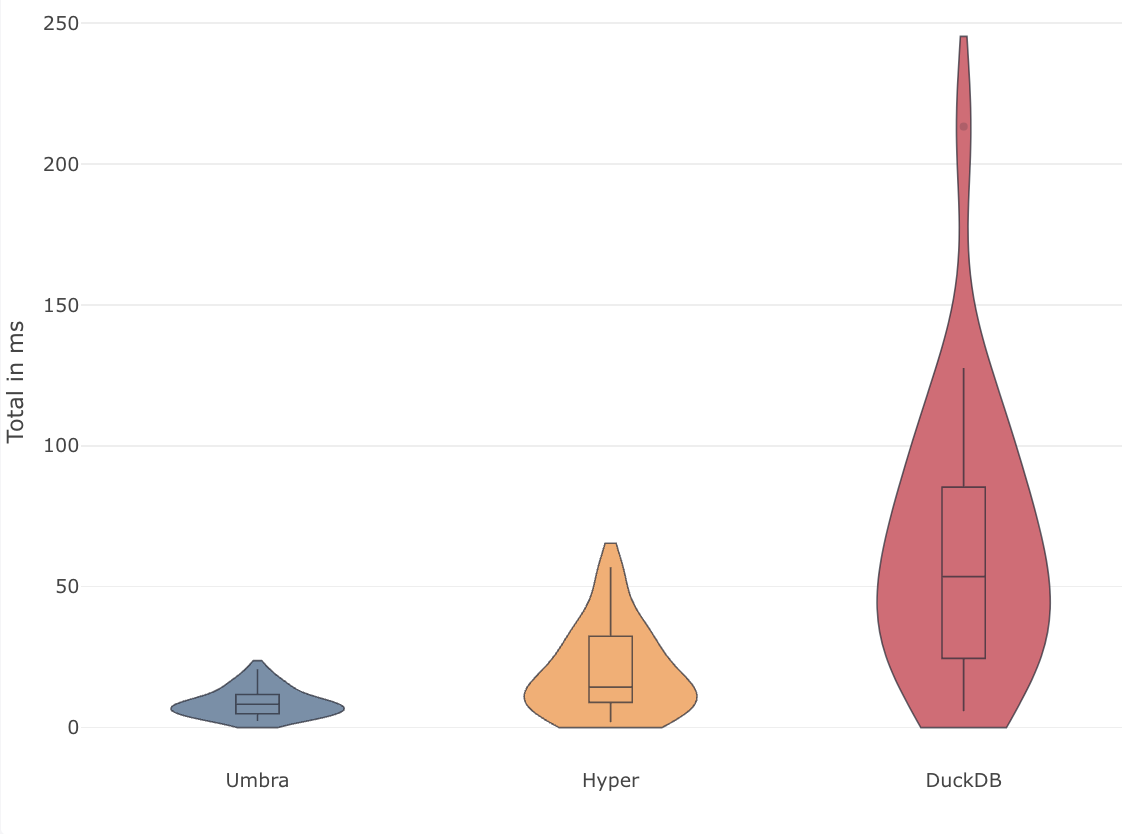
\includegraphics[width=\linewidth]{figures/scale-linear.png}
    \caption{Violin plot with linear scale.}
      \label{fig:scale-linear}
  \end{subfigure}
  \hspace{0.5cm} % Adjust the horizontal space between the figures
  \begin{subfigure}[b]{0.3\linewidth}
    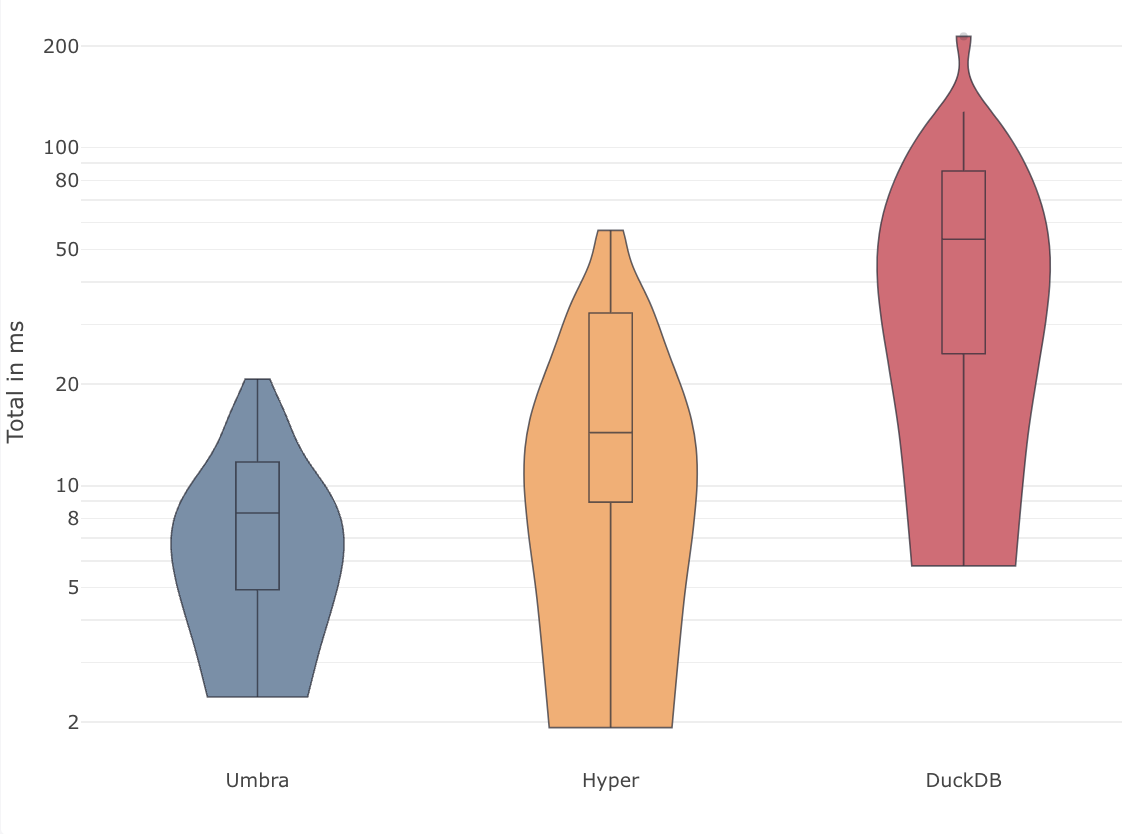
\includegraphics[width=\linewidth]{figures/scale-log.png}
    \caption{Violin plot with logarithmic scale.}
      \label{fig:scale-log}
  \end{subfigure}
  \hspace{0.5cm} % Adjust the horizontal space between the figures
  \begin{subfigure}[b]{0.3\linewidth}
    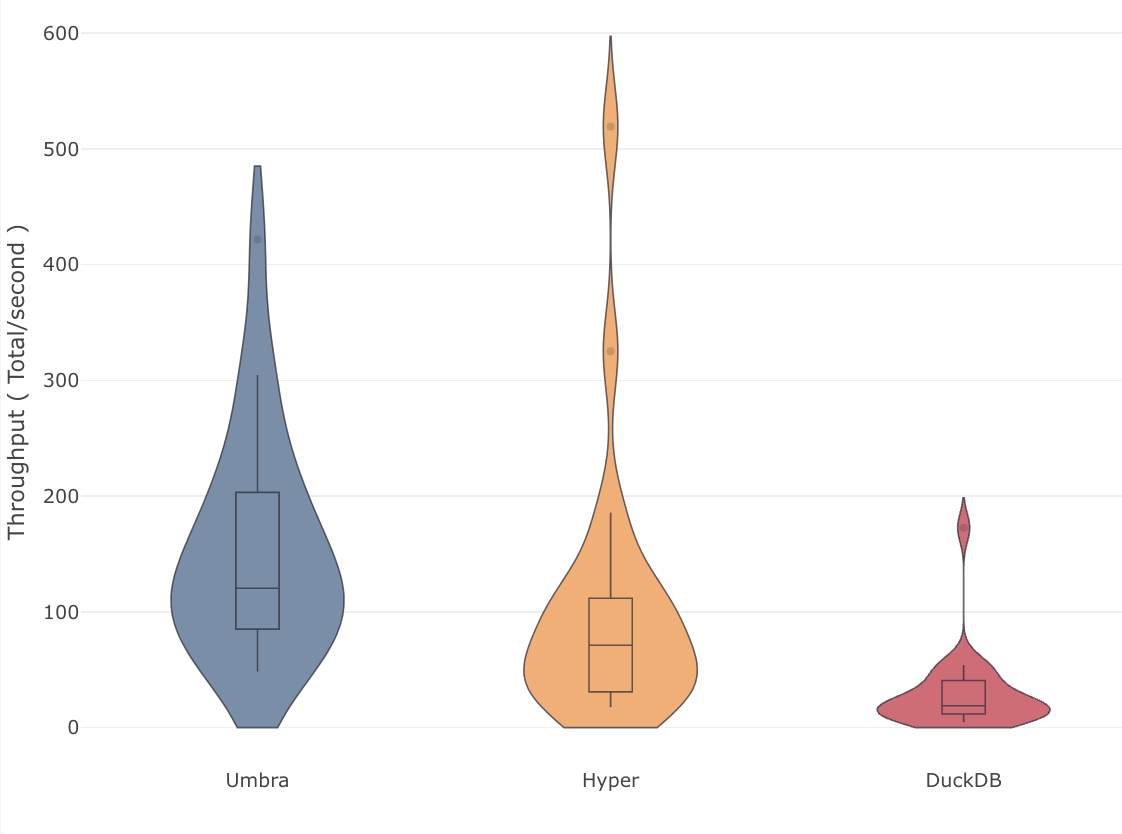
\includegraphics[width=\linewidth]{figures/scale-throughput.png}
    \caption{Violin plot with throughput based scale.}
      \label{fig:scale-throughput}
  \end{subfigure}
  \caption{Comparison of violin plots using different scales: A visual representation of the same dataset, highlighting how variations appear under linear, logarithmic, and throughput scaling.}
  \label{fig:scale-comparison.}
\end{figure}

The logarithmic scale excels in highlighting proportional changes across a wide range of values. This is particularly advantageous when dealing with datasets that span several orders of magnitude, ensuring that both small and large values are perceptible.

The throughput scale is specifically designed for scenarios where the emphasis is on the rate of data transfer or processing. It provides a unique perspective, crucial in benchmarking scenarios where throughput is a critical performance metric.

By seamlessly switching between these Y-axis types globally, users can extract diverse insights from the same set of data, enhancing the versatility and depth of their analytical processes.


% - Violin: scatter und boxplot
The Benchy Viewer also offers customization options for violin plots. Users can choose between representing data inside the violins as individual data points or as a boxplot, as illustrated in Figure~\ref{fig:chart-configuration-violin}. Opting for data points means that each query data is individually represented, providing a wealth of detailed information. On the other hand, selecting the "Boxplot" option replaces individual data points with a summarized boxplot inside the violin. This option streamlines the visualization, offering clarity by presenting an overview of the data distribution. Users have the flexibility to tailor the representation based on their specific analytical needs.

\begin{figure}[h]
  \centering
  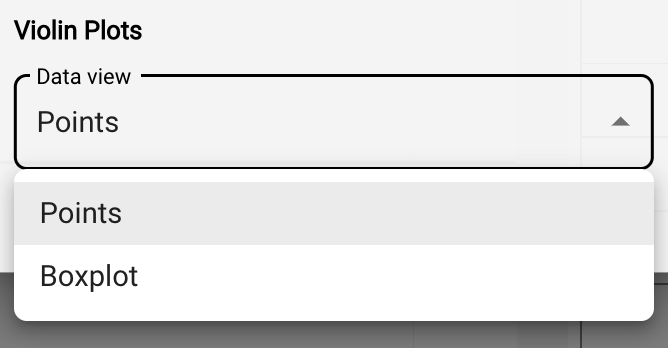
\includegraphics[width=0.4\linewidth]{figures/chart-configuration-violin.png}
  \caption{Drop-down menu of global options, offering the selection of displaying data points or a boxplot within the violins of the violin charts.}
  \label{fig:chart-configuration-violin}
\end{figure}

\subsection{Saving and Sharing the Application State}\label{sec:saving-sharing-state}

One of the valuable features of the Benchy Viewer is its ability to save and share the application state. This encompasses all configurations related to visualization elements, global options, and dashboard settings. Users can conveniently save their current setup or download it for future reference, as depicted in Figure~\ref{fig:save-upload}.

\subsubsection{Downloading Configuration}
The saved configurations can be downloaded as a file, allowing users to keep a record of specific setups or share them with colleagues. This downloaded file serves as a snapshot of the application state at the time of saving.

\subsubsection{Uploading Configurations}
To recreate a previous analysis session, users can upload a saved configuration file. This action loads all the configurations, restoring the dashboard layout, applied visualizations, and global settings. It's a time-saving feature that ensures a seamless transition back to a specific analytical context.


\begin{figure}[h]
  \vspace{0.5cm}
  \centering
  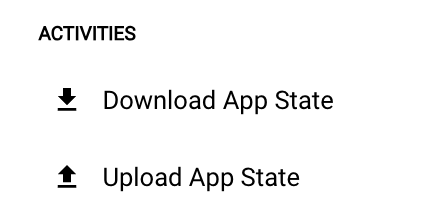
\includegraphics[width=0.4\linewidth]{figures/save-upload.png}
  \caption{Downloading and uploading the application state.}
  \label{fig:save-upload}
\end{figure}


\subsubsection{Facilitating Collaboration}
The ability to share configuration files promotes collaboration among users. Team members can easily exchange analysis setups, ensuring a consistent view of data and enabling more effective collaboration on complex analytical projects.

In essence, the "Saving and Sharing" feature enhances the flexibility and collaborative potential of the Benchy Viewer, providing users with a convenient way to exchange analytical contexts.
